\documentclass[10pt,a4paper]{article}
\usepackage[utf8]{inputenc}
\usepackage{amsmath}
\usepackage{amsfonts}
\usepackage{amssymb}
\usepackage{graphicx}
\usepackage{epstopdf}
\usepackage{inputenc}
\usepackage{geometry}
\usepackage{graphicx}
\usepackage[normalem]{ulem}
\usepackage{hyperref}
\usepackage{enumitem}
\usepackage[dvipsnames]{xcolor}
\usepackage{subcaption}
\hypersetup{
    colorlinks=false, %set true if you want colored links
    linktoc=all,     %set to all if you want both sections and subsections linked 
}
\author{Author: \textcolor{MidnightBlue}{\href{https://www.linkedin.com/in/simone-staffa-8b3b79158}{Simone Staffa}}}
\title{{\Huge\textbf{Process and Service Design}
\\ \LARGE Professor: Pierluigi Plebani
\begin{figure}[h!]
 \hfill 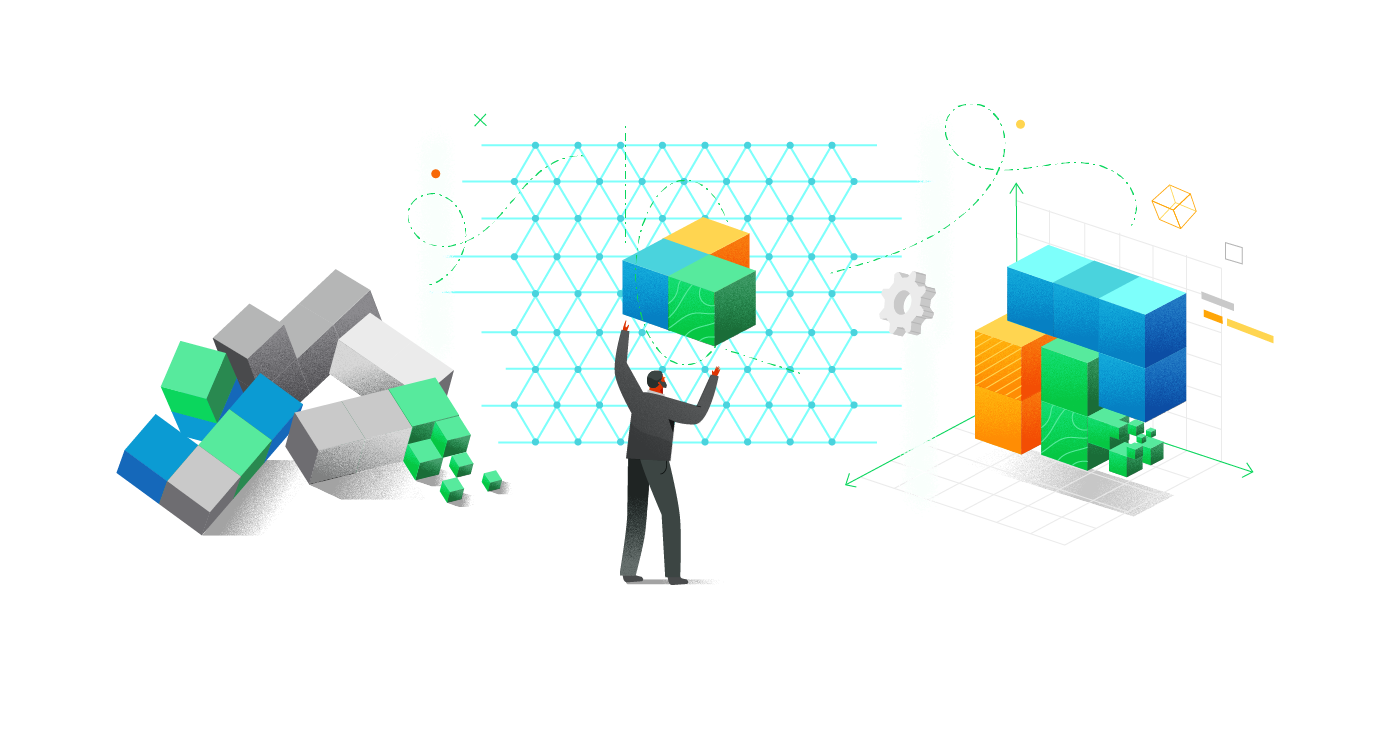
\includegraphics[width=200pt]{images/cover.png}\hspace*{\fill}
  \label{fig:polimi}
\end{figure} \\
}}
\date{Politecnico di Milano \\ Computer Science $\&$ Engineering | Fall 2019-2020}
\newcommand{\mydefinition}[1]{\textcolor{MidnightBlue}{\textit{"#1"}\\ \\}}
\newcommand{\myparagraph}[1]{\paragraph{\uline{#1}}\mbox{}\\[0.05in]}
\begin{document}
\maketitle
\clearpage
\tableofcontents
\clearpage
\section{\LARGE Introduction}
The meaning of term \textbf{service} is intuitive but is definition can be different in different contexts like:
\begin{itemize}
	\item Economic
	\item ICT
\end{itemize}
We firstly need to understand similarities and differences among these different terms:
\begin{itemize}
	\item Service
	\item e-Service
	\item Web-Service
\end{itemize}
\uline{Definition of service (economic perspective)}: \\
\textit{“A service is a change in the condition of a person, or a good belonging to some economic unit, which is brought about as the result of the activity of some other economic unit, with the prior agreement of the former person or economic unit,"  (P. Hill, On goods and services)} \\
\begin{figure}[h!]
  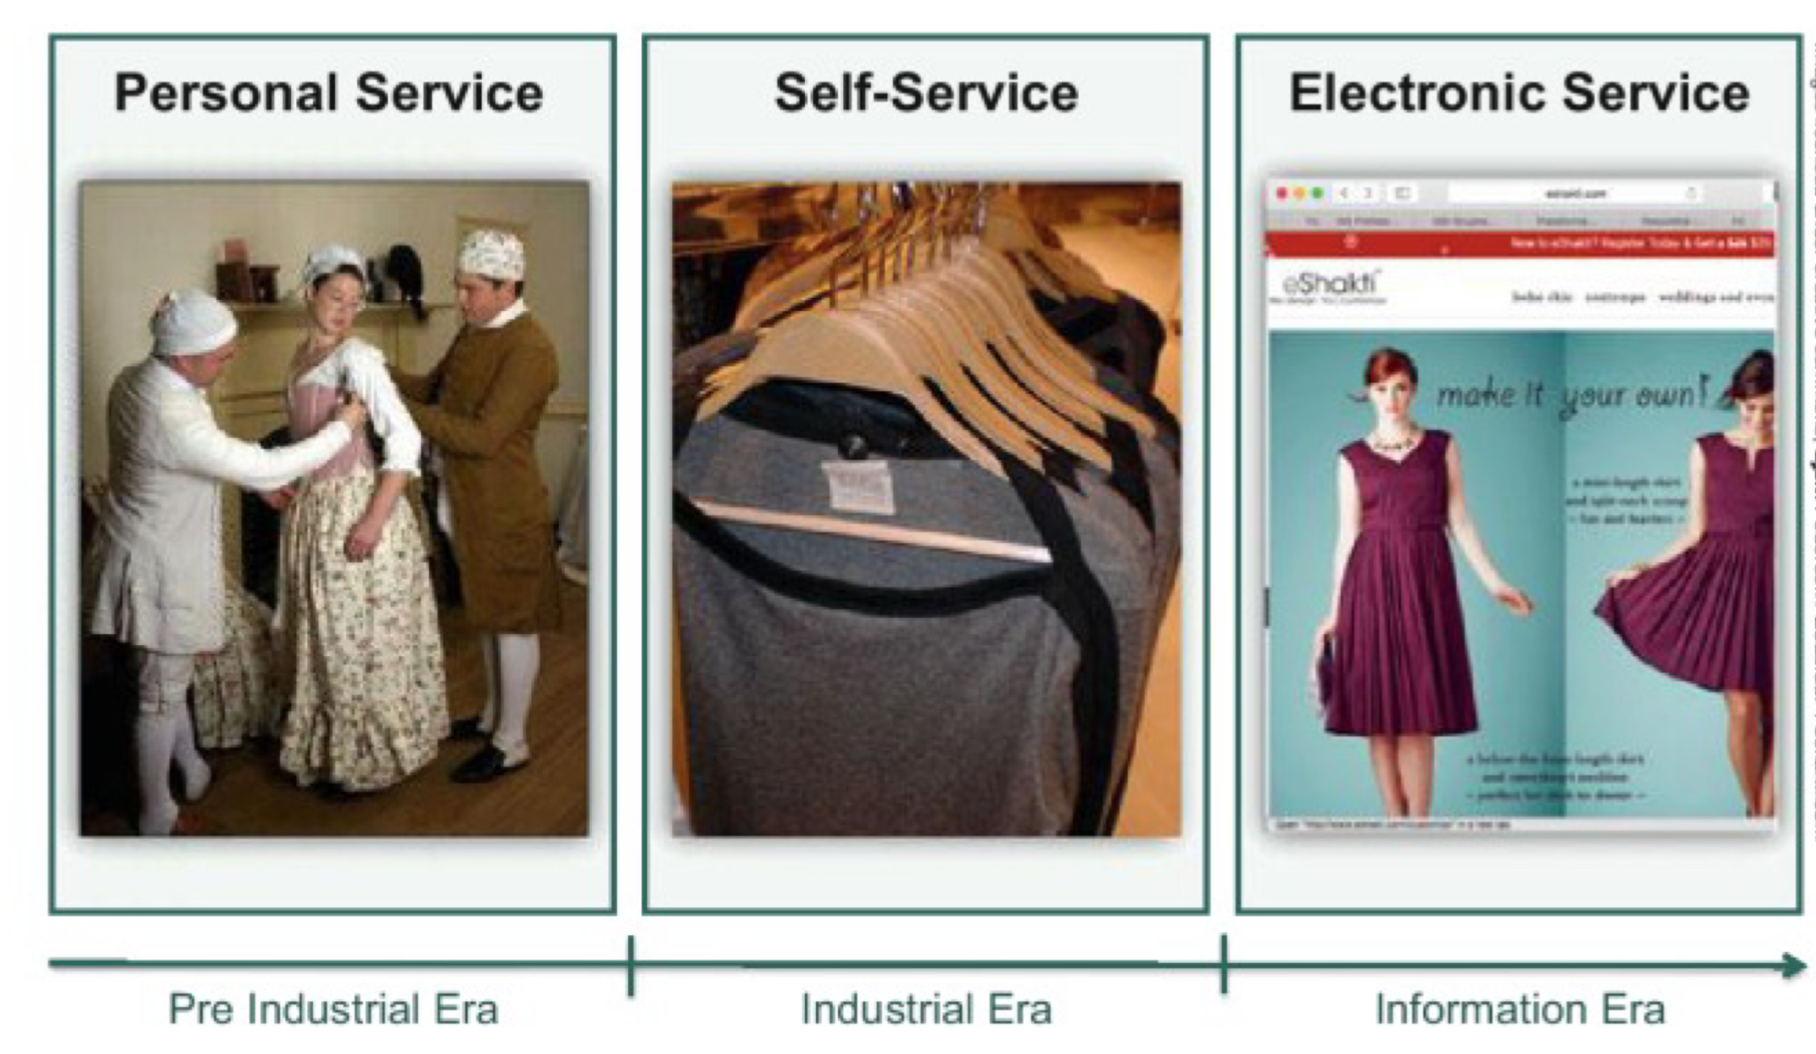
\includegraphics[width=\linewidth]{images/services-types}
  \caption{Looking for a dress, in different eras}
  \label{fig:service-eras}
\end{figure} \\
The above picture represents the evolution of the services along the years. Specially, it refers to the dress service. In the Pre Industrial era was more like a personal service, where a tailors offered totally customized dresses to people directly in their houses. Then with the Industrial Era, dresses were sold by retailer, so the final product was not really customized by the consumers, who just had to select the already made dress they liked. Finally, nowadays in the Information Era, service started to be offered through IT Platforms, with full customization without even the need to go to the shop, dresses can be just bought and received at home.\\
This can be also applied to the IT domain, for what we call nowadays Web Services. \\
The Pre Industrial Era corresponds to when people used to build their own computers, buying different parts and installing them by their selves. The Industrial Era corresponds to when companies started building personal computers to be sold to consumers, who just had to pay and bring them home. Finally, the Information Era corresponds to nowadays Cloud Platform and Web Services that allow people to rent virtual computers online, to perform their own computation. \\ \\
Just to recap:
\begin{itemize}
	\item \textbf{Personal service (Pre Industrial era)}: highly and man-made customization but limited production
	\item \textbf{Industrial service (Industrial era)}: mass production but no customization
	\item \textbf{Electronic service (Information era)}: highly and computer-based customization combined with mass production
\end{itemize}
This to say that we are \textbf{evolving to a service-oriented society}. \\
\uline{\textit{"We don't need a drill, we need a hole in the wall."}} \\ \\ 
From an economic perspective, we are switching from a Good-dominant logic to a Service-dominant logic.
\begin{itemize}
	\item \textbf{Good-dominant logic} focuses on goods exchange, that's why goods are considered to be tangible and each of them has an embedded value that is taken into account to operate exchange transactions.
	\item \textbf{Service-dominant logic} focuses on service provision, where resources are  intangible and require a co-creation of value.
\end{itemize}
S-D logic is useful because it opens to more interactions with customers and allows to focus on why a product fits to the customer needs instead of technical specification. \\ \\
When technology comes into play, there are two different perspectives of ICT in S-D logic, which go under the name of e-Service.
\begin{itemize}
	\item As the improvement of a programming paradigm
	\begin{itemize}
		\item \textbf{ICT is a goal} and it is offered itself as a service
		\item SOA (Service Oriented Architecture) becomes the new way of developing software to be service-ready
		\end{itemize}
\item As the automation of economics activities and self-service
	\begin{itemize}
		\item \textbf{ICT is a mean} and can improve the effectiveness and the efficacy
		\item The goal is to make the business able to provide services
	\end{itemize}
\end{itemize}
As a mean, ICT has a fundamental role in the evolution towards the S-D logic. Who deliver products must pay a lot of attention on Customization, Scalability, Reliability and Security/Privacy. \\
As a goal, ICT is also a service to be delivered and a possible way to deliver these service could be using a Web Service.
\section{\LARGE Service Definition}
\uline{Definition of service (IT perspective)}: \\
\textit{“A service is a mechanism to enable access to one or more capabilities, where the access is provided using a prescribed interface and is exercised consistent with constraints and policies as specified by the service description. A service is provided by an entity – the service provider – for use by others, but the eventual consumers of the service may not be known to the service provider and may demonstrate uses of the service beyond the scope originally conceived by the provider.”  (P. Hill, On goods and services)} \\ \\
\subsection{Software Oriented Architecture}
\textbf{Service-Oriented Architecture (SOA)} is a style of software design where services are provided to the other components by application components, through a communication protocol over a network. In service oriented architecture, a number of services communicate with each other, in one of two ways: through passing data or through two or more services coordinating an activity. \\
\subsubsection{Reference Model}
SOA in the end is a \uline{reference model}. A reference model is an abstract \textbf{framework} for understanding significant relationships among the entities of some environment. It enables the development of specific reference or concrete architectures using consistent standards or specifications supporting that environment. A reference model consists of a minimal set of unifying concepts, axioms and relationships withing a particular problem domain, and is independent of specific standards, technologies, implementations, or the concrete details. \\ \\
Following discussion on SOA RM is taken from [1]
\subsubsection{SOA Reference Model}
The goal of this reference model is to define the essence of service oriented architecture, and emerge with a vocabulary and a common understanding of SOA. 
\begin{figure}[h!]
 \hfill 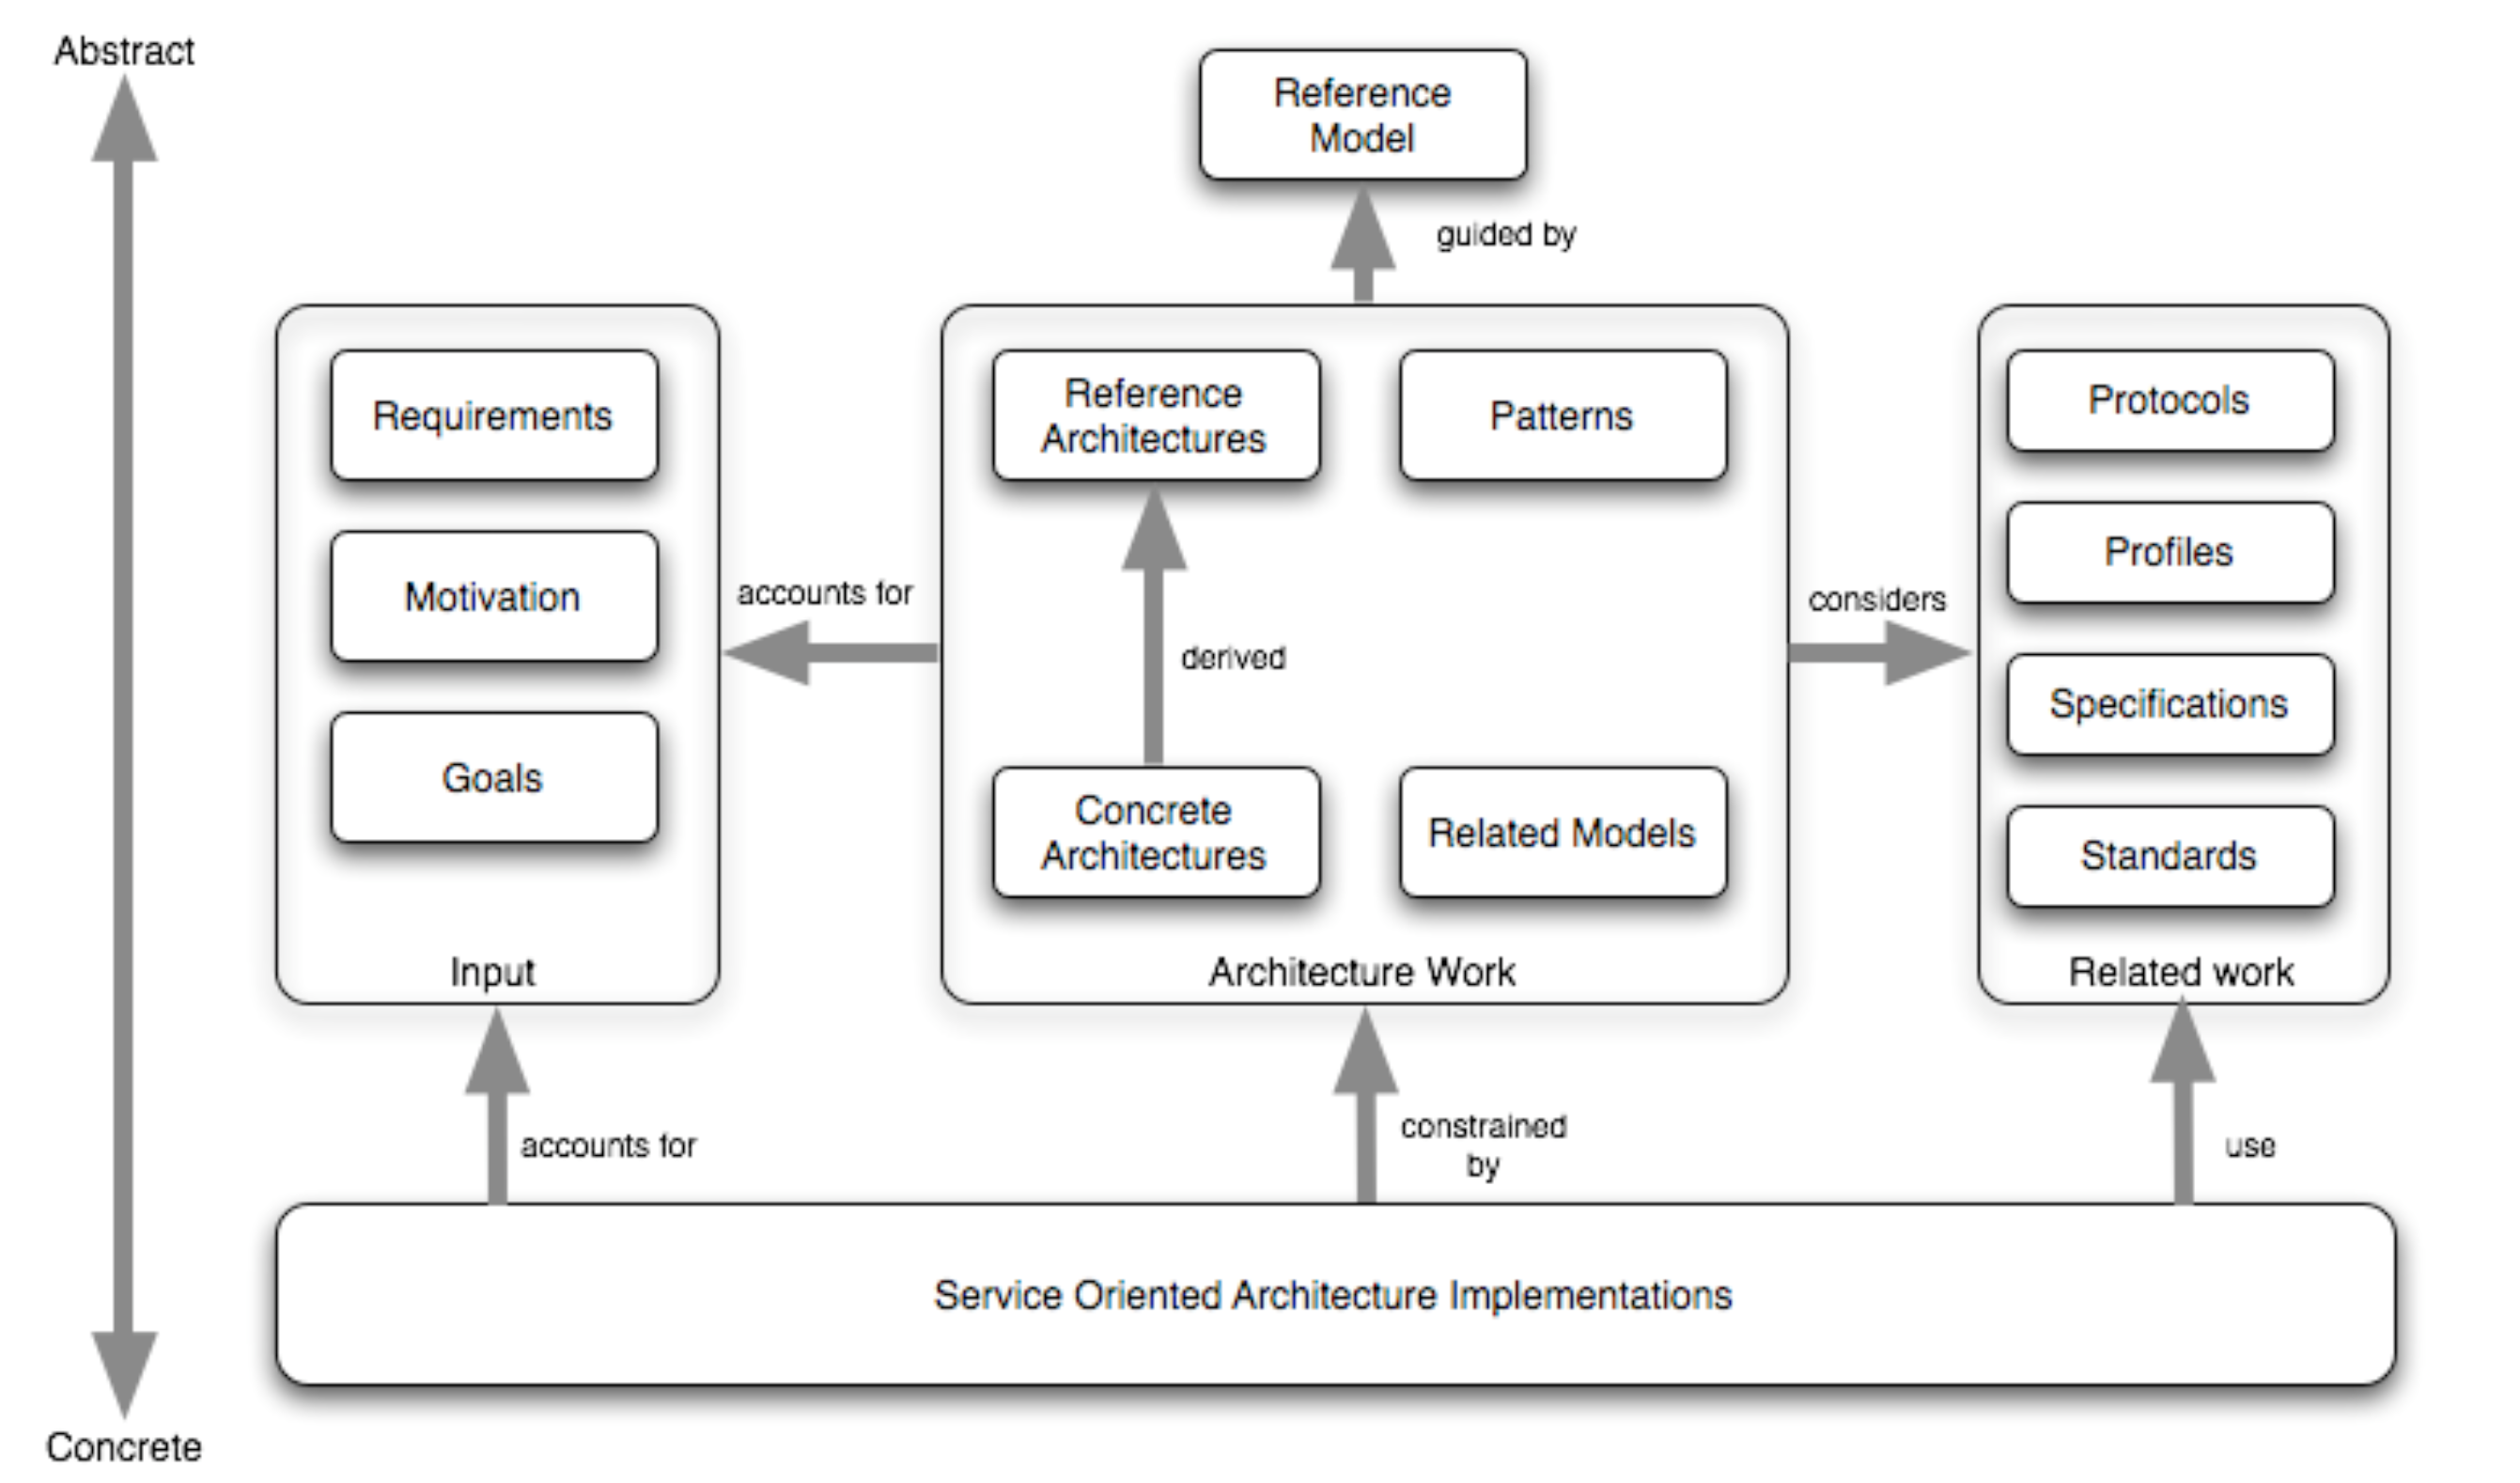
\includegraphics[width=180pt]{images/soa-rm}\hspace*{\fill}
  \caption{How the Referenced Model relates to other work}
  \label{fig:soa-rm}
\end{figure}  \\
Figure 2 shows how a reference model for SOA relates to other distributed systems architectural inputs. The concepts and relationships defined by the reference model are intended to be the basis for describing references architectures and patterns that will define more specific categories of SOA designs. Concrete architectures arise from a combination of reference architectures, architectural patterns and additional requirements, including those imposed by technology environments.
\subsubsection{What is Service Oriented Architecture}
Service Oriented Architecture is a paradigm for organizing and utilizing distributed capabilities that may be under the control of different ownership domains. \\
In general, entities (people and organizations) create capabilities to solve or support a solution for the problems they face in the course of their business. It is natural to think of one person’s needs being met by capabilities offered by someone else; or, in the world of distributed computing, one computer agent’s requirements being met by a computer agent belonging to a different owner. \\ The perceived value of SOA is that it provides a powerful framework for matching needs and capabilities and for combining capabilities to address those needs. \\ \\
Visibility, interaction, and effect are key concepts for describing the SOA paradigm. \textbf{Visibility} refers to the capacity for those with needs and those with capabilities to be able to see each other. This is typically done by providing descriptions.\\ \textbf{Interaction} is the activity of using a capability. Typically mediated by the exchange of messages, an interaction proceeds through a series of information exchanges and invoked actions. This permits service providers and consumers to interact and provides a decision point for any policies and contracts that may be in force. \\ \\
The purpose of using a capability is to realize one or more \textbf{real world effects}. At its core, an interaction is "an act" as opposed to "an object" and the result of an interaction is an effect. This effect may be the return of information or the change in the state of entities (known or unknown) that are involved in the interaction. \\ \\ We are careful to distinguish between \textit{public} actions and \textit{private} actions; private actions are inherently unknowable by other parties. On the other hand, public actions result in changes to the \textit{state} that is shared between at least those involved in the current execution context and possibly shared by others. Real world effects are, then, couched in terms of changes to this \textbf{shared state}. \\ \\
This description of SOA has yet to mention what is usually considered the central concept: the \textbf{service}. The noun "service" is defined in dictionaries as "The performance of work (a function) by one for another". \\
While both needs and capabilities exist independently of SOA, \textbf{in SOA services are the mechanism by which needs and capabilities are brought together.} \\ \\ SOA is a means of organizing solutions that promotes reuse, growth and interoperability. It is an organizing and delivery paradigm that enables one to get more value from use both of capabilities which are locally "owned" and those under the control of others. \\ \\
The concepts of visibility, interaction, and effect apply directly to services in the same manner as these were described for the general SOA paradigm. Visibility is promoted through the service description which contains the information necessary to interact with the service and describes this in such terms as the service inputs, outputs, and associated semantics. The service description also conveys what is accomplished when the service is invoked and the conditions for using the service. \\ \\ In general, entities (people and organizations) offer capabilities and act as service providers. Those with needs who make use of services are referred to as service consumers. 
\subsubsection{Benefits of SOA}
The value of SOA is that it provides a simple scalable paradigm for organizing large networks of systems that require interoperability to realize the value inherent in the individual components. Indeed, SOA is scalable because it makes the fewest possible assumptions about the network and also minimizes any trust assumptions that are often implicitly made in smaller scale systems. \\ \\ Through this inherent ability to scale and evolve, SOA enables an IT portfolio which is also adaptable to the varied needs of a specific problem domain or process architecture. The infrastructure SOA encourages is also more agile and responsive than one built on an exponential number of pair-wise interfaces. Therefore, SOA can also provide a solid foundation for business agility and adaptability.
\subsection{The Reference Model}
\begin{figure}[h!]
 \hfill 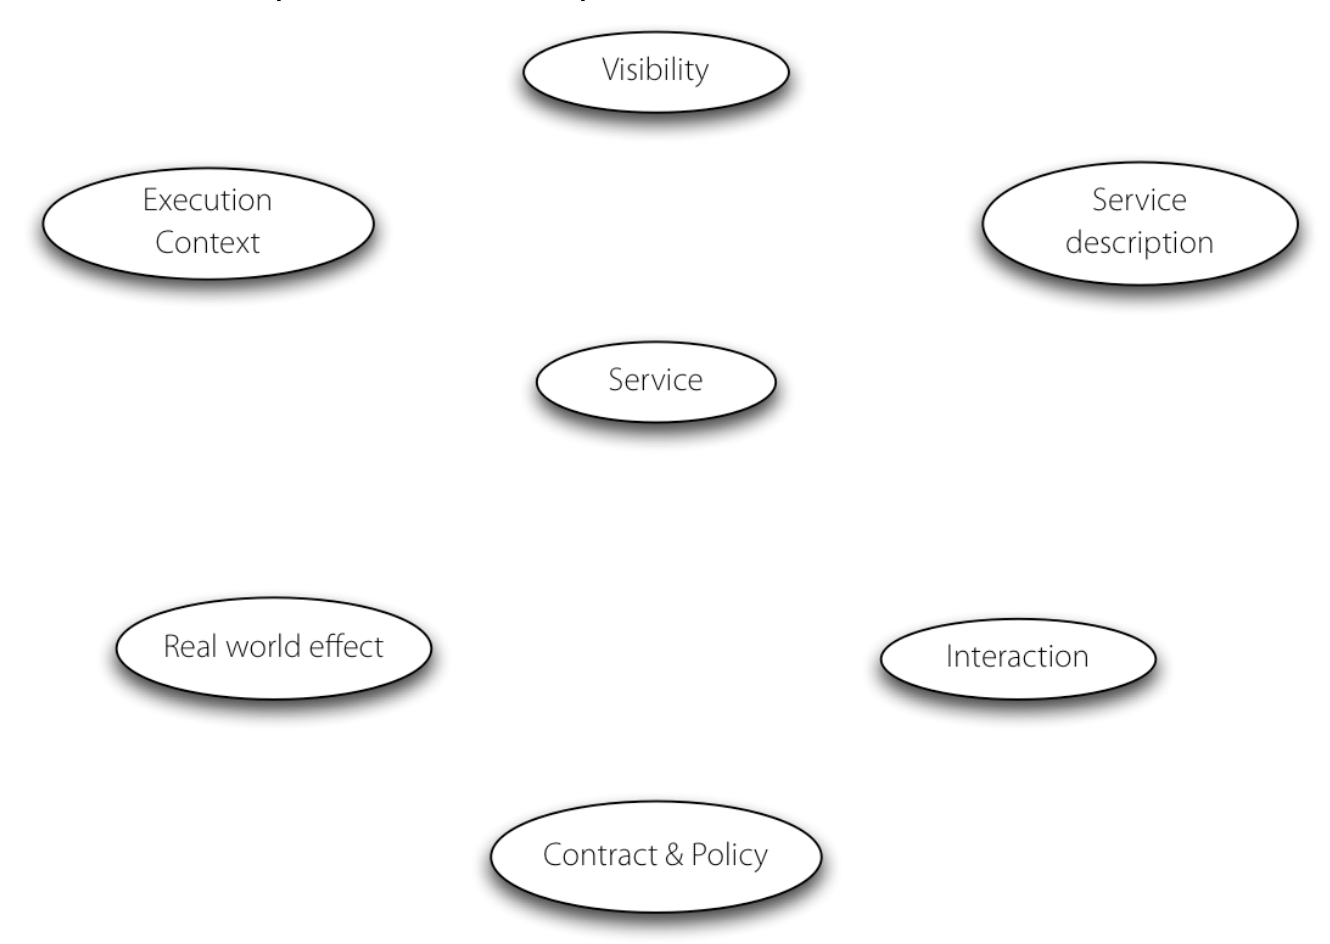
\includegraphics[width=160pt]{images/rm}\hspace*{\fill}
  \caption{Principal concepts in the Reference Model}
  \label{fig:reference-model}
\end{figure} 
\subsubsection{Service}
A service is a mechanism to enable access to one or more capabilities, where the access is provided using a prescribed interface and is exercised consistent with constraints and policies as specified by the service description. A service is provided by an entity – the \textbf{service provider} – for use by others, but the eventual consumers of the service may not be known to the service provider and may demonstrate uses of the service beyond the scope originally conceived by the provider. A service is accessed by means of a service interface, where the interface comprises the specifics of how to access the underlying capabilities. \\ \\
A service is opaque in that its implementation is typically hidden from the service consumer except for (1) the information and behavior models exposed through the service interface and (2) the information required by service consumers to determine whether a given service is appropriate for their needs. \\ \\
The consequence of invoking a service is a realization of one or more real world effects. These effects may include:
\begin{enumerate}
	\item Information returned in response to a request for that information
	\item A change to the shared state of defined entities
	\item A combination of (1) and (2)
\end{enumerate}
\subsubsection{Dynamics of Services}
From a dynamic perspective, there are three fundamental concepts that are important in understanding what is involved in interacting with services: the visibility between service providers and consumers, the interaction between them, and the real world effect of interacting with a service.
\begin{figure}[h!]
 \hfill 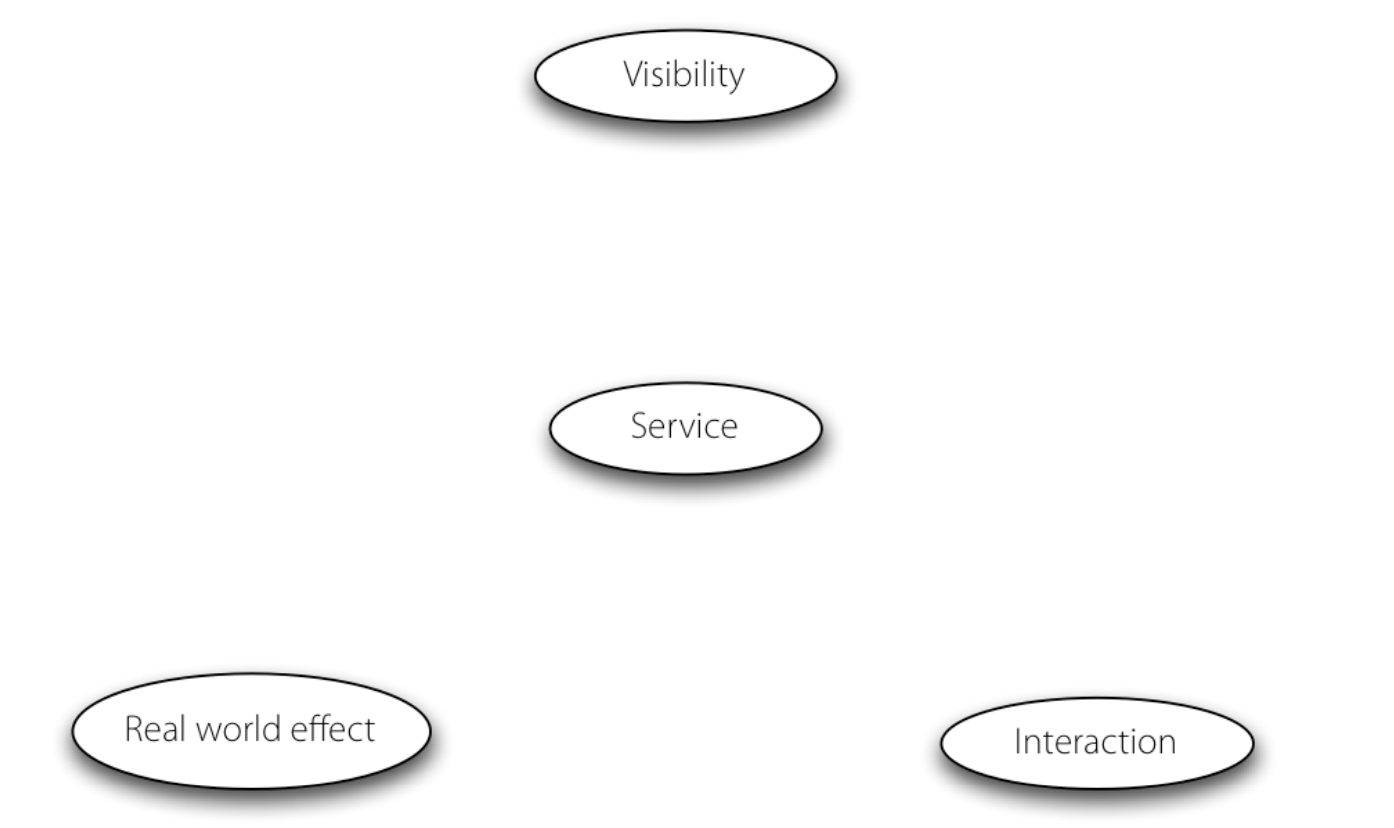
\includegraphics[width=180pt]{images/dynamics-services}\hspace*{\fill}
  \caption{Concepts around the dynamics of a service}
  \label{fig:dynamics}
\end{figure} 
\myparagraph{Visibility}
 For a service provider and consumer to interact with each other they have to be able to "see" each other. This is true for any consumer/provider relationship. In the case of SOA, visibility needs to be emphasized because it is not necessarily obvious how service participants can see each other. \\
 Preconditions to visibility are awareness, willingness and reachability. The initiator MUST be aware of the other parties, the participants MUST be predisposed to interaction, and the participants must be able to interact.
 \begin{itemize}
 	\item \textbf{Awareness}: both the service provider and the service consumer MSUT have information that would lead them to know of the other's existence. Awareness of service offerings is often effected by various \textit{discovery} mechanisms. For a service consumer to discover a a service, the service provider must be capable of making details (service description and policies) of the service available to potential consumers.
 	\item \textbf{Willingness}: t is an intentional act to initiate and to participate in a service interaction. For example, if a service consumer discovers a service via its description in a registry, and the consumer initiates an interaction, if the service provider does not cooperate then there can be no interaction. The extent of a service participant's willingness to engage in service interactions may be the subject of policies. 
 	\item \textbf{Reachability}: the relationship between service participants where they are able to interact; possibly by exchanging information. This is an essential pre-requisite for service interaction - participants MUST be able to communicate with each other. A service consumer may have the intention of interacting with a service, however, if the service is not reachable, the service would not be visible by the consumer.
 \end{itemize}
 \myparagraph{Interaction}
Interacting with a service involves performing actions against the service. In many cases, this is accomplished by sending and receiving messages, but there are other modes possible that do not involve explicit message transmission. For example, a service interaction may be effected by modifying the state of a shared resource. However, for simplicity, we often refer to message exchange as the primary mode of interaction with a service.
\begin{figure}[h!]
 \hfill 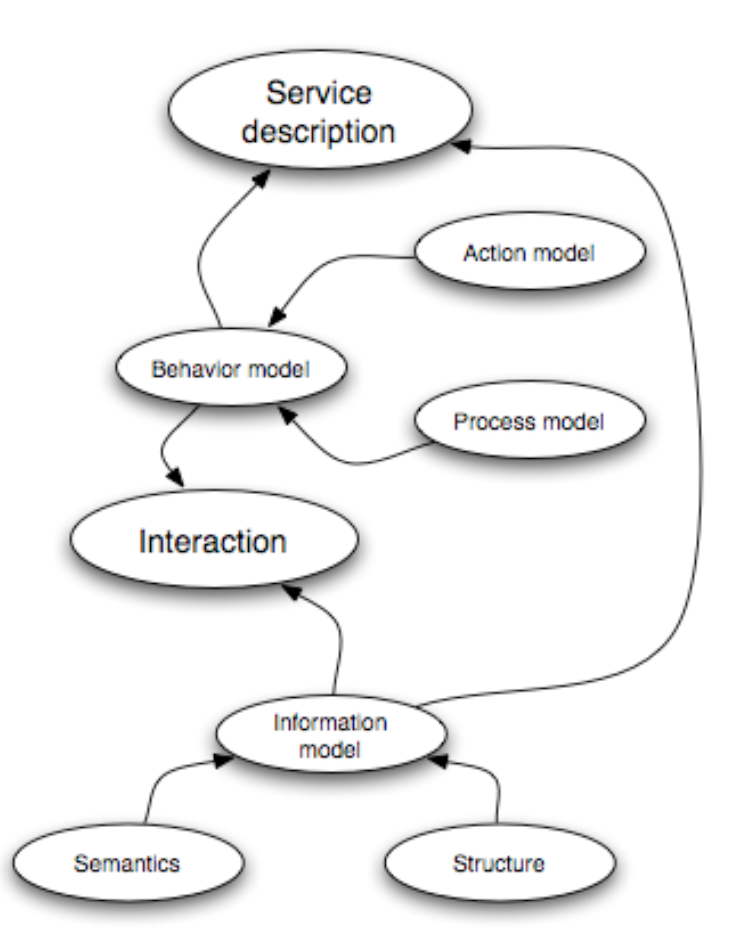
\includegraphics[width=185pt]{images/interaction}\hspace*{\fill}
  \caption{Service Interaction concepts}
  \label{fig:interaction}
\end{figure}  \\
Figure 5 illustrates the key concepts that are important in understanding what it is involved in interacting with services; these revolve around the service description – which references a information model and a behavior model.
\begin{itemize}
	\item \textbf{Information model}: a characterization of the information that may be exchanged with the service. Only information and data that are potentially exchanged with a service are generally included within that service's information model. The scope of the information model includes the format of information that is exchanged, the structural relationships within the exchanged information and also the definition of terms used. Knowing the representation, structure, and form of information required is a key initial step in ensuring effective interactions with a service. There are several levels of such structural information; including the encoding of character data, the format of the data and the structural data types associated with elements of the information.
	\item \textbf{Behavior model}: knowledge of the actions invoked against the service and the process or temporal aspects of interacting with the service. This is characterized as knowledge of the actions on, responses to, and temporal dependencies between actions on the service. For example, in a security-controlled access to a database, the actions available to a service consumer include presenting credentials, requesting database updates and reading results of queries. The \uline{action model} of a service is the characterization of the actions that may be invoked against the service. The \uline{process model} characterizes the temporal relationships and temporal properties of actions and events associated with interacting with the service.
\end{itemize}
\myparagraph{Real World Effect}
There is always a particular purpose associated with interacting with a service. Conversely, a service provider (and consumer) often has a priori conditions that apply to its interactions. The service consumer is trying to achieve some result by using the service, as is the service provider. At first sight, such a goal can often be expressed as “trying to get the service to do something”. This is sometimes known as the “real world effect” of using a service. For example, an airline reservation service can be used to learn about available flights, seating and ultimately to book travel – the desired real world effect being information and a seat on the right flight.
\\ As previously stated, a real world effect can be the response to a request for information or the change in the state of some defined entities shared by the service participants. In this context, the shared state does not necessarily refer to specific state variables being saved in physical storage but rather represents shared information about the affected entities.
\begin{figure}[h!]
 \hfill 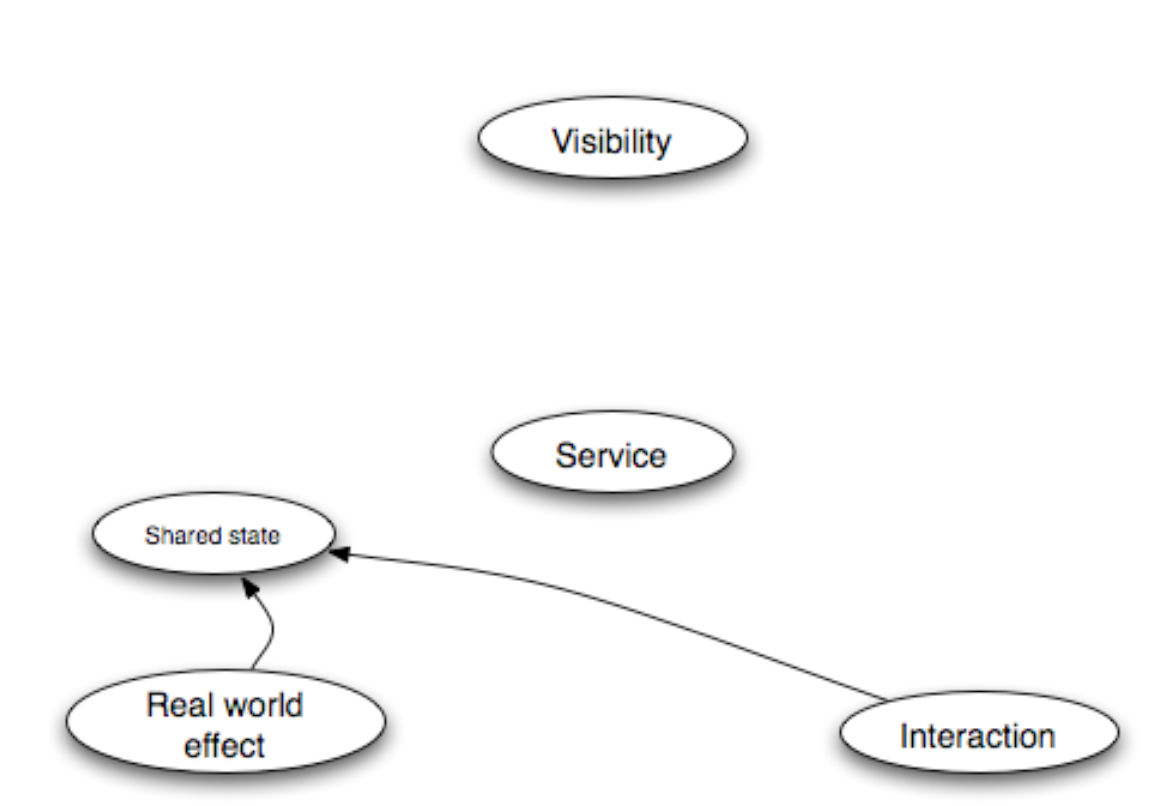
\includegraphics[width=180pt]{images/real-world-effect}\hspace*{\fill}
  \caption{Real World Effect and shared state}
  \label{fig:real-world-effect}
\end{figure}  \\
In addition, the internal actions that service providers and consumers perform as a result of participation in service interactions are, by definition, private and fundamentally unknowable. By unknowable we mean both that external parties cannot see others’ private actions and, furthermore, SHOULD NOT have explicit knowledge of them. Instead we focus on the set of facts shared by the parties – the shared state. Actions by service providers and consumers lead to modifications of this shared state; and the real world effect of a service interaction is the accumulation of the changes in the shared state. \\ \\
For example, when an airline has confirmed a seat for a passenger on a flight this represents a fact that both the airline and the passenger share – it is part of their shared state. Thus the real world effect of booking the flight is the modification of this shared state – the creation of the fact of the booking. Flowing from the shared facts, the passenger, the airline, and interested third parties may make inferences – for example, when the passenger arrives at the airport the airline confirms the booking and permits the passenger onto the airplane (subject of course to the passenger meeting the other requirements for traveling). \\ For the airline to know that the seat is confirmed it will likely require some private action to record the reservation. However, a passenger should not have to know the details of the airline internal procedures. Likewise, the airline does not know if the reservation was made by the passenger or someone acting on the passenger’s behalf. The passenger’s and the airline’s understanding of the reservation is independent of how the airline maintains its records or who initiated the action.
\subsubsection{About services}
In support of the dynamics of interacting with services are a set of concepts that are about services themselves. These are the service description, the execution context of the service and the contracts and policies that relate to services and service participants.
\begin{figure}[h!]
 \hfill 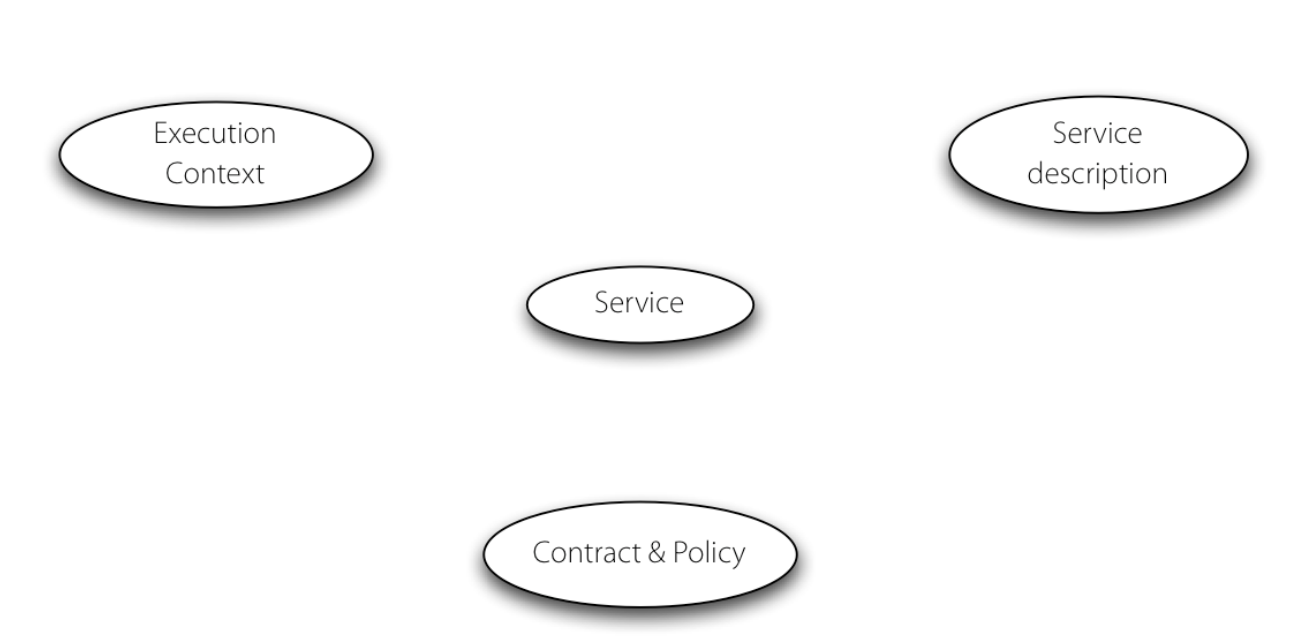
\includegraphics[width=180pt]{images/about-services}\hspace*{\fill}
  \caption{About services}
  \label{fig:about-services}
\end{figure}
\myparagraph{Service description}
The service description represents the information needed in order to use a service. In most cases, there is no one “right” description but rather the elements of description required depend on the context and the needs of the parties using the associated entity. While there are certain elements that are likely to be part of any service description, most notably the information model, many elements such as function and policy may vary.
\begin{figure}[h!]
 \hfill 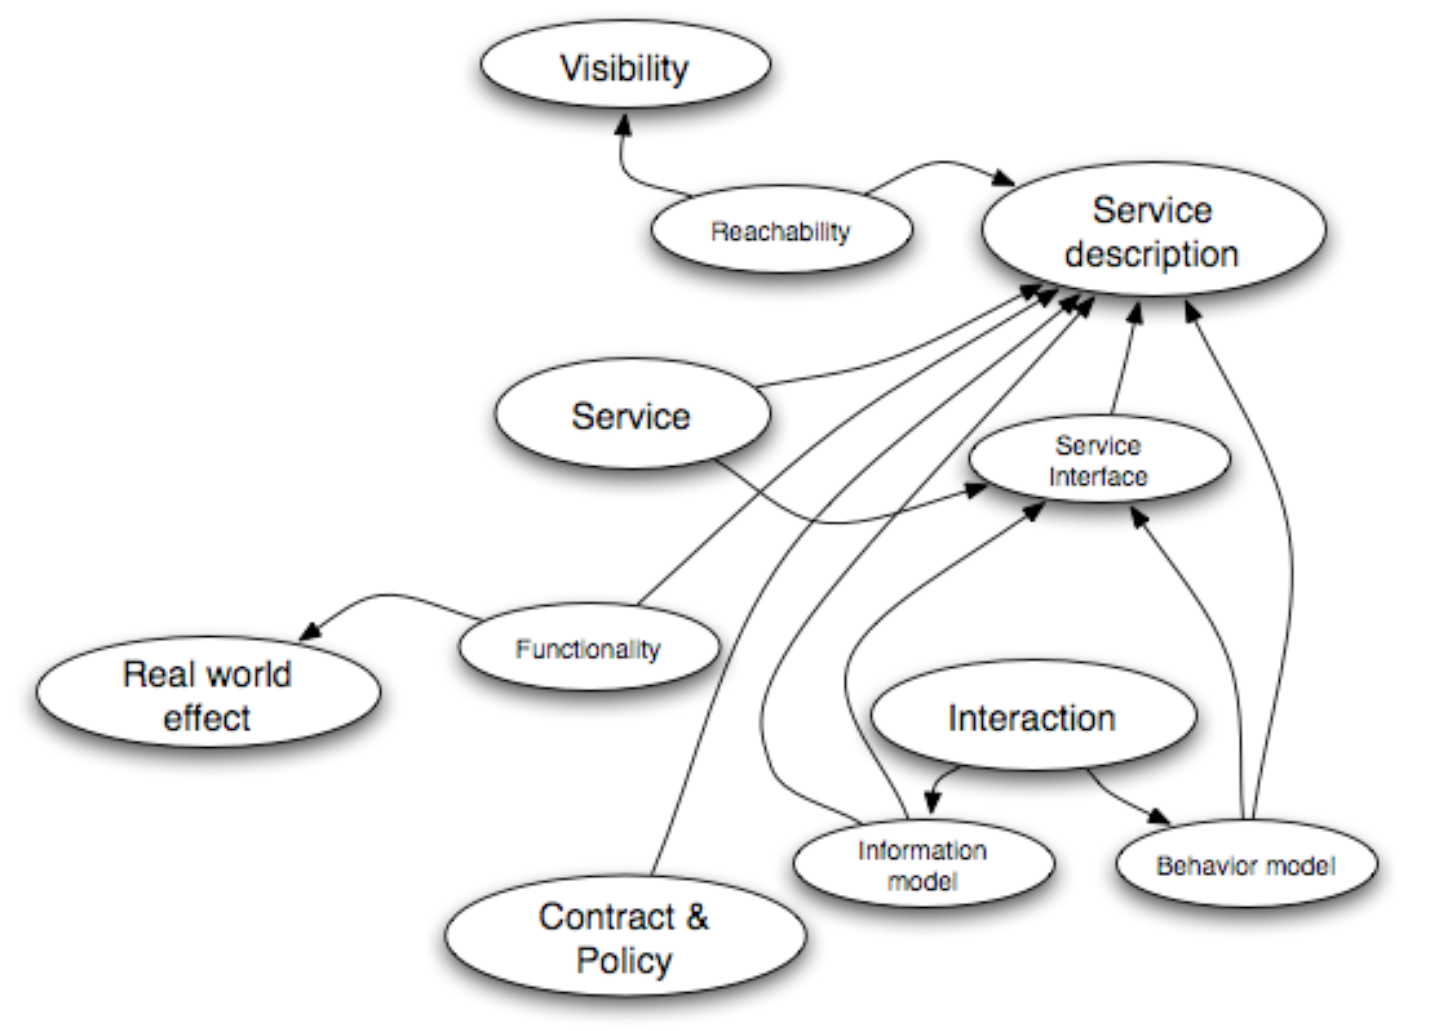
\includegraphics[width=180pt]{images/service-description}\hspace*{\fill}
  \caption{Service description}
  \label{fig:description}
\end{figure}
The purpose of description is to facilitate interaction and visibility, particularly when the participants are in different ownership domains, between participants in service interactions. By providing descriptions, it makes it possible for potential participants to construct systems that use services and even offer compatible services. Best practice suggests that the service description SHOULD be represented using a standard, referenceable format. \\ \\
The service description makes available critical information that a consumer needs in order to decide whether or not to use a service. In particular, a service consumer needs to possess the following items of information:
\begin{enumerate}
	\item That the service exists and is \textbf{reachable}
	\item That the service performs a certain function or set of functions
	\item That the service operates under a specified set of constraints and policies
	\item That the service will (to some implicit or explicit extent) comply with policies as prescribed by the service consumer
	\item How to interact with the service in order to achieve the required objectives, including the format and content of information exchanged between the service and the consumer and the sequences of information exchange that may be expected
\end{enumerate}
\subparagraph{Service Reachability}
Reachability is an inherently pairwise relationship between service providers and service consumers. However, a service description SHOULD include sufficient data to enable a service consumer and service provider to interact with each other. This MAY include metadata such as the location of the service and what information protocols it supports and requires. It MAY also include dynamic information about the service, such as whether it is currently available.
\subparagraph{Service Functionality}
A service description SHOULD unambiguously express the function(s) of the service and the real world effects that result from it being invoked. The description of functionality may include, among other possibilities, a textual description intended for human consumption or identifiers or keywords referenced to specific machine-processable definitions. Part of the description of functionality may include underlying technical assumptions that determine the limits of functionality exposed by the service or of the underlying capability.
\subparagraph{Policies Related to a Service}
A service description MAY include support for associating policies with a service and providing necessary information for prospective consumers to evaluate if a service will act in a manner consistent with the consumer’s constraints.
\subparagraph{Service Interface}
The service interface is the means for interacting with a service. It includes the specific protocols, commands, and information exchange by which actions are initiated that result in the real world effects as specified through the service functionality portion of the service description. The specifics of the interface SHOULD be syntactically represented in a standard referenceable format. These prescribe what information needs to be provided to the service in order to access its capabilities and interpret responses. This is often referred to as the service’s information model. it is assumed that for a service to be usable, its interface MUST be represented in a format that allows interpretation of the interface information by its consumers.
\pagebreak
\myparagraph{Policies and Contracts}
A \uline{policy} represents some constraint or condition on the use, deployment or description of an owned entity as defined by any participant. A \uline{contract}, on the other hand, represents an agreement by two or more parties. Like policies, agreements are also about the conditions of use of a service.
\begin{figure}[h!]
 \hfill 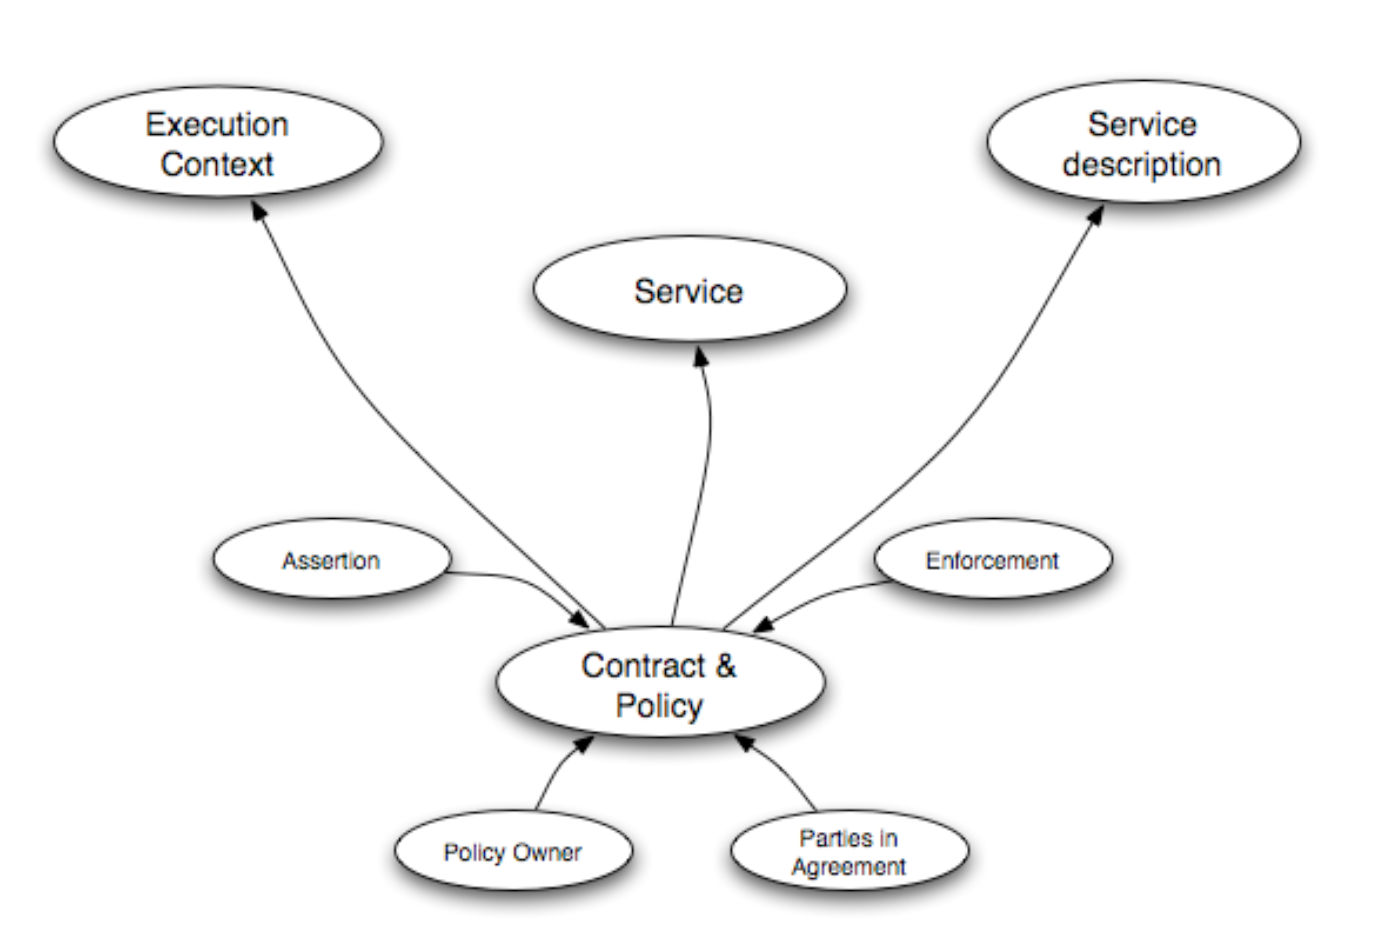
\includegraphics[width=180pt]{images/policies-contracts}\hspace*{\fill}
  \caption{Policies and Contracts}
  \label{fig:policies-and-contracts}
\end{figure}
\subparagraph{Service Policy}
Conceptually, there are three aspects of policies: the policy assertion, the policy owner (sometimes referred to as the policy subject) and policy enforcement.
\begin{itemize}
	\item \textbf{Policy Assertion}: for example, the assertion: “All messages are encrypted” is an assertion regarding the forms of messages. As an assertion, it is measurable: it may be true or false depending on whether the traffic is encrypted or not. Policy assertions are often about the way the service is realized; i.e., they are about the relationship between the service and its execution context.
	\item \textbf{Policy Enforcement}: techniques for the enforcement of policies depend on the nature of the policy. Conceptually, service policy enforcement amounts to ensuring that the policy assertion is consistent with the real world. This might mean preventing unauthorized actions to be performed or states to be entered into; it can also mean initiating compensatory actions when a policy violation has been detected.
\end{itemize}
Policies potentially apply to many aspects of SOA: security, privacy, manageability, Quality of Service and so on. Beyond such infrastructure-oriented policies, participants MAY also express business-oriented policies – such as hours of business, return policies and so on.
\subparagraph{Service Contract}
Whereas a policy is associated with the point of view of individual participants, a contract represents an agreement between two or more participants. Like policies, contracts can cover a wide range of aspects of services: quality of service agreements, interface and choreography agreements and commercial agreements. Note that we are not necessarily referring to legal contracts here. \\ \\
Thus, following the discussion above, a service contract is a measurable assertion that governs the requirements and expectations of two or more parties. Unlike policy enforcement, which is usually the responsibility of the policy owner, contract enforcement may involve resolving disputes between the parties to the contract. The resolution of such disputes may involve appeals to higher authorities.
\pagebreak
\myparagraph{Execution Context}
\begin{figure}[h!]
 \hfill 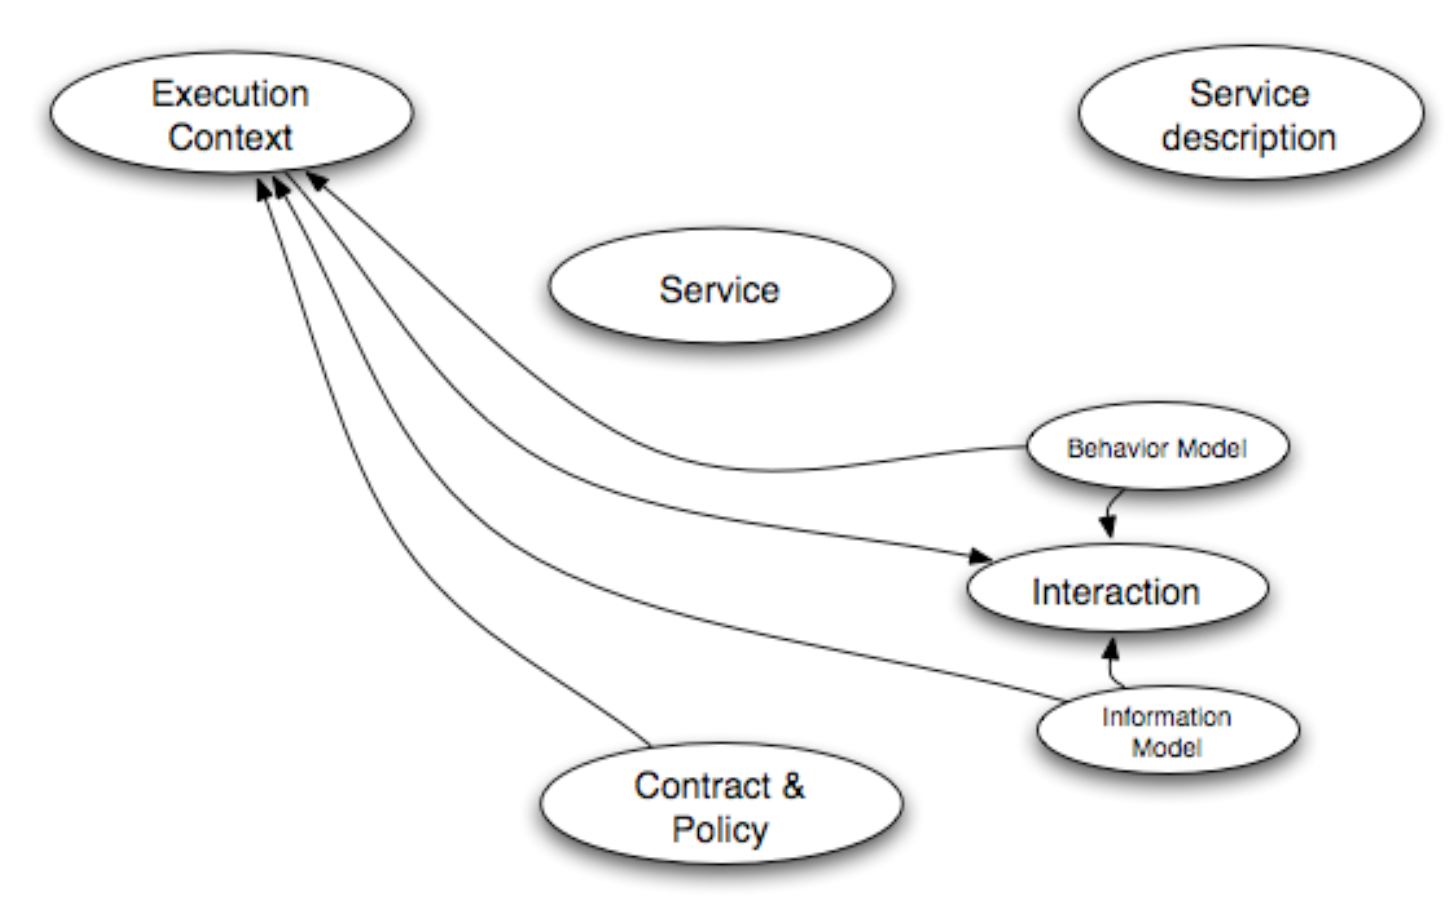
\includegraphics[width=180pt]{images/execution-context}\hspace*{\fill}
  \caption{Execution Context}
  \label{fig:execution-context}
\end{figure} \\
The execution context of a service interaction is the set of infrastructure elements, process entities, policy assertions and agreements that are identified as part of an instantiated service interaction, and thus forms a path between those with needs and those with capabilities. \\ \\
As discussed in previous sections of this document, the service description (and a corresponding description associated with the service consumer and its needs) contains information that can include preferred protocols, semantics, policies and other conditions and assumptions that describe how a service can and may be used.
The participants (providers, consumers, and any third parties as noted below) must agree and acknowledge a consistent set of agreements in order to have a successful service interaction, i.e. realizing the described real world effects. The execution context is the collection of this consistent set of agreements. \\ \\
The consumer and provider can be envisioned as separate places on a map and, for a service to actually be invoked, a path must be established between those two places. This path is the execution context. \\ \\
The execution context also allows us to distinguish services from one another. Different instances of the same service – denoting interactions between a given service provider and different service consumers for example – are distinguished by virtue of the fact that their execution contexts are different. \\ \\
Finally, the execution context is also the context in which the interpretation of data that is exchanged takes place. A particular string has a particular meaning in a service interaction in a particular context – the execution context.
\pagebreak
\subsubsection{IBM SOA Reference Architecture}
\begin{figure}[h!]
 \hfill 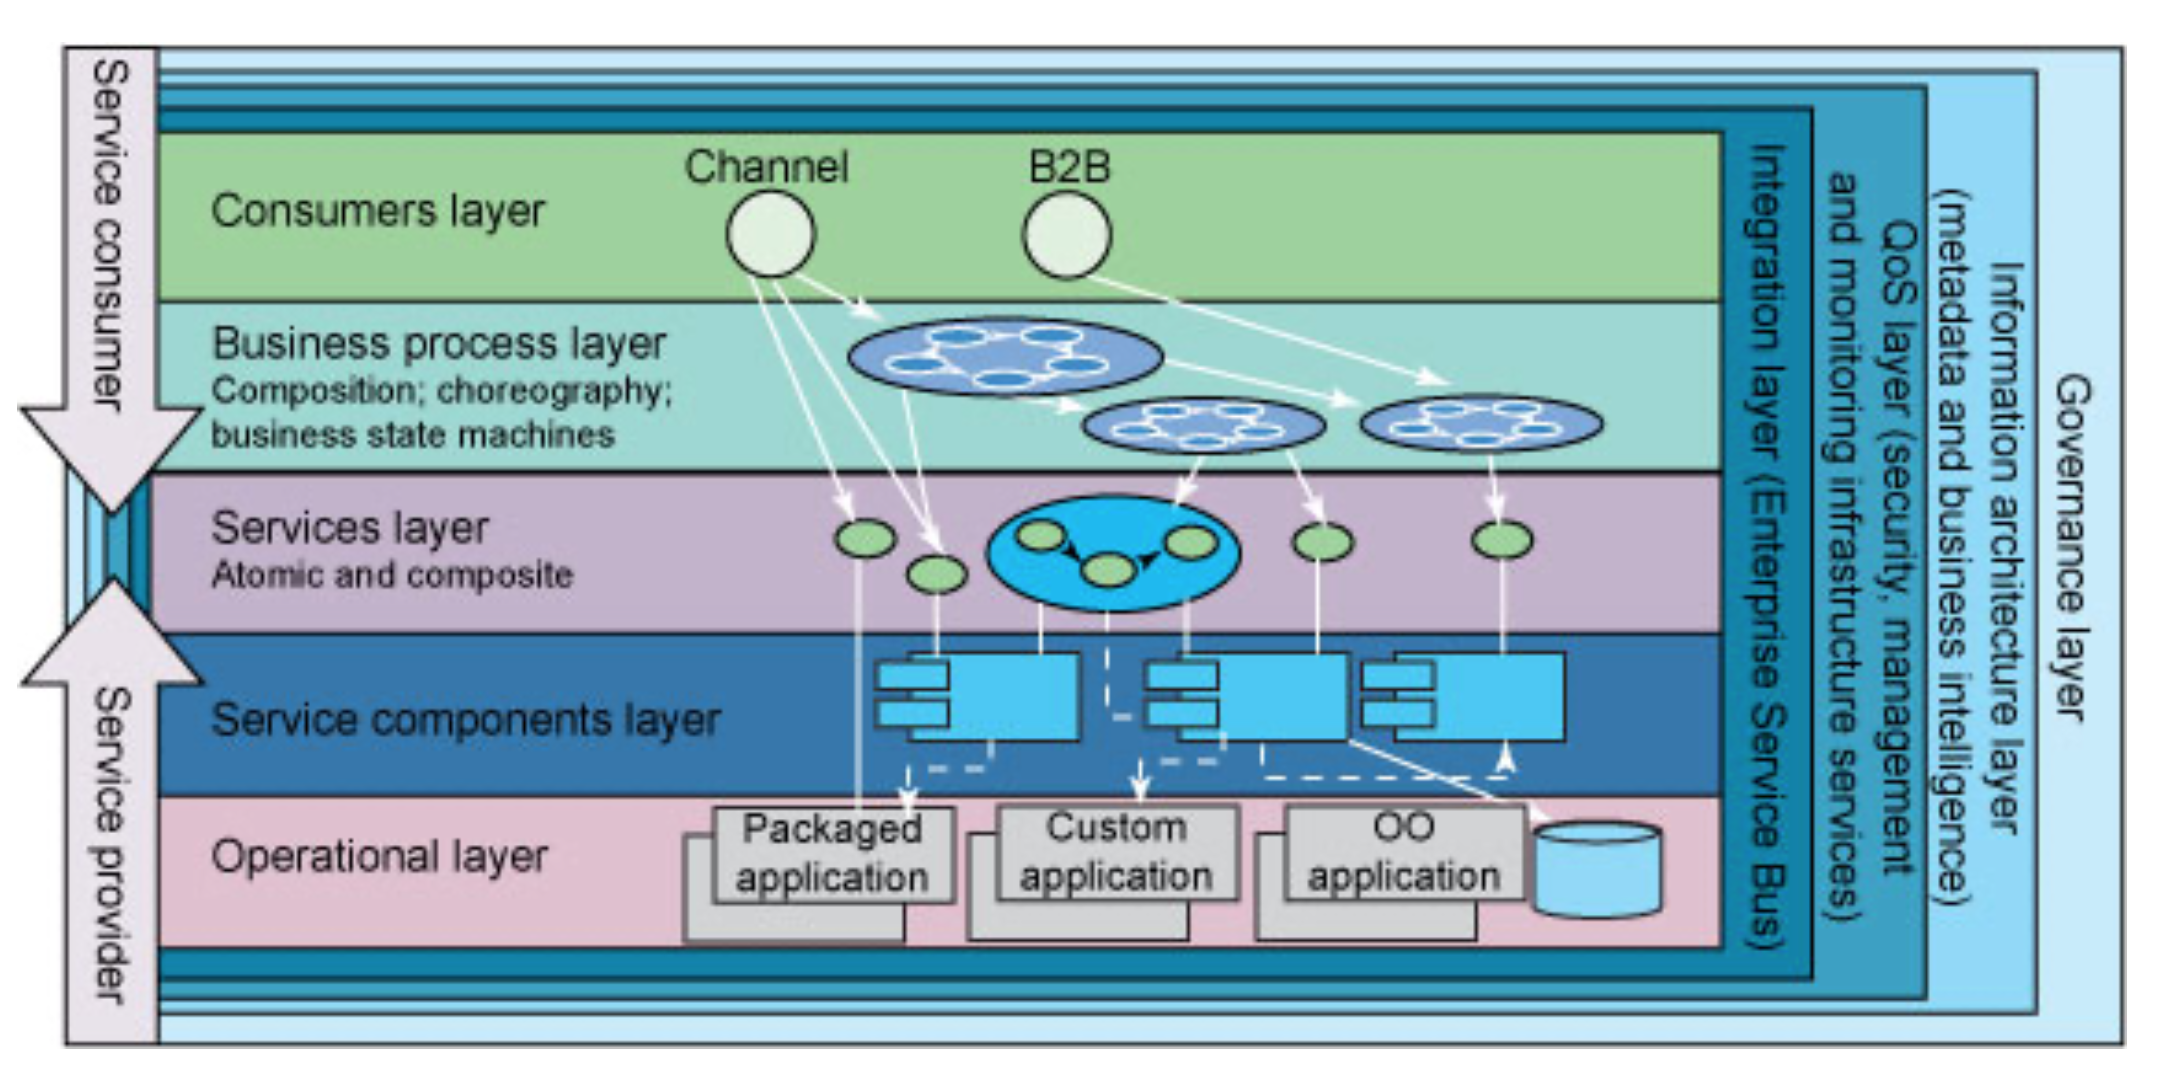
\includegraphics[width=\linewidth]{images/ibm-soa}\hspace*{\fill}
  \caption{IBM SOA Reference Architecture}
  \label{fig:imb-soa}
\end{figure}
The SOA RA allows architects to use its contents such as the building blocks as a checklist of elements: architectural building blocks and their relations in each layer, the options available, decisions that need to be made at each layer. The layers provide a starting point for the separation of concerns needed to build an SOA. Each group of the separated concerns are represented in their own "layer." \\ \\
Within each of the layers depicted in Figure 11 there are Architectural Building Blocks (ABBs) that represents a basic element of reusable functionality and fulfill the key responsibilities of that layer. Each ABB resides in a layer, supports capabilities, and has responsibilities. ABBs are also connected to one another across the layers and provide a natural association between layers. If a particular connection between ABBs occurs consistently across layers to solve a certain problem this then defines a pattern of ABBs as well as the valid interaction sequences between the architectural building blocks. \\ \\
Along with the ABBs there are also the capabilities that they support. A capability is defined by the Open Group in TOGAF 9, as "an ability that an organization, person, or system possesses". So, expanding on that definition, ABBs provide the technical resource to allow an organization, person or system to be able to provide their defined capability. An ABB, providing support for one or more capabilities, that can be realized by one or more components or products; examples of the responsibilities of an ABB include: service definition, mediation, routing, etc.
\pagebreak
\myparagraph{Summary of the layers}
First, as we can see from Figure 11, there are some layers that are visible only to service providers and some visible only to service consumers which are Operational Layer + Service Components Layer and Consumers Layer + Business Process Layer respectively. Then in the middle we have the Service Layer which is the only one visible to both actors. \\
The layers that are defined in an SOA RA are as follows:
\begin{itemize}
	\item \textbf{Operational Layer}: captures the organization's infrastructure, both new and existing, needed to support the SOA solution at design, deploy and run time. This layer represents the intersection point between the actual runtime infrastructure and the rest of the SOA which runs on that infrastructure. In addition, it is the integration point for an underlying Infrastructure as a Service (IaaS) construct and the rest of the SOA in the wider context of cloud computing.
	\item \textbf{Service Component Layer}: contains software components, each of which provide the implementation or "realization" for a service, or operation on a service. The layer also contains the functional and technical components that facilitate a Service Component to realize one or more services. Software components hide the complexity of the underlying system and exposes with standard interface what defined in the Service Layer Its aim is to satisfy the Service Level Agreements.
	\item \textbf{Service Layer}: consists of all the logical services defined within the SOA. This layer contains the descriptions for services, business capabilities, and IT manifestation that are used/created during design time as well as service contracts and descriptions that are used at runtime. Here service consumer is able to read the service description, while the service provider can decide to offer service components 'as-ease' or can combine services to create something new to offer.
	\item \textbf{Business Process Layer}: covers the process representation, composition methods, and building blocks for aggregating loosely coupled services as a sequenced process aligned with business goals. Data flow and control flow are used to enable interactions between services and business processes. The role of this layer is central in pursuing the Business-IT alignment. Service consumer here can compose services using two strategies: orchestration and choreography. 
	\item \textbf{Consumer Layer}: is the point where consumers, whether if be a person, program, browser or automation, interact with the SOA. It enables an SOA solution to support a client-independent, channel agnostic set of functionality, which is separately consumed and rendered through one or more channels (client platforms and devices). This layer provides the capability to quickly create the front end of the business processes and composite applications in order to respond to changes in the marketplace.
	\item \textbf{Integration Layer}:  is a cross-cutting concern that enables and provides the capability to mediate, which includes transformation, routing and protocol conversion to transport service requests from the service requester to the correct service provider.
	\item \textbf{Quality of Service Layer}: is a cross-cutting concern that supports non functional requirement (NFR) related concerns of an SOA and provides a focal point for dealing with them in any given solution. It provides the means of ensuring that an SOA meets its requirements with respect to: monitoring, reliability, availability, manageability, transactionality, maintainability, scalability, security, safety, life cycle, etc.
	\item \textbf{Information Architecture Layer}: is a cross-cutting concern that is responsible for manifesting a unified representation of the information aspect of an organization as provided by its IT services, applications, and systems enabling business needs and processes and aligned with the business vocabulary. This layer includes information architecture, business analytics and intelligence.
	\item \textbf{Governance Layer}: is a cross-cutting concern that ensures that the services and SOA solutions within an organization are adhering to the defined policies, guidelines and standards that are defined as a function of the objectives, strategies and regulations applied in the organization and that an SOA solutions are providing the desired business value.
\end{itemize}
\subsection{e-Service}
A service is an activity (not necessarily atomical) that can be more or less complex, so it may imply the existence of a process. A service involces two actors: 
\begin{itemize}
	\item \textbf{Service provider}
	\item \textbf{Service consumer}
\end{itemize}
A service provider may become a service consumer and the vice-versa. \\ 
A service requires a prior agreement. Usually service exchanges last longer than good exchange and the interaction between providers and consumer could be complex. \\ \\
\textit{“Service systems comprise service providers and service clients working together to co-produce value in complex value chains or networks.”} (S. Vargo, R. Lusch)\\ \\
Co-creation implies that customers and providers are not fixed roles: provider may become customer of someone else and a customer may become a provider. \\
Service system can be more o r less complex involving a different number of actors, that's why governance of a service network is not an easy task.
\subsubsection{Customers and providers interaction}
There are different scenarios according to the involvement of persons and their belongings.
\myparagraph{Person acting on person}
A person delivers a service to another person and no belongings are involved on both sides. Note that this scenario is not interesting to us.
\begin{figure}[h!]
 \hfill 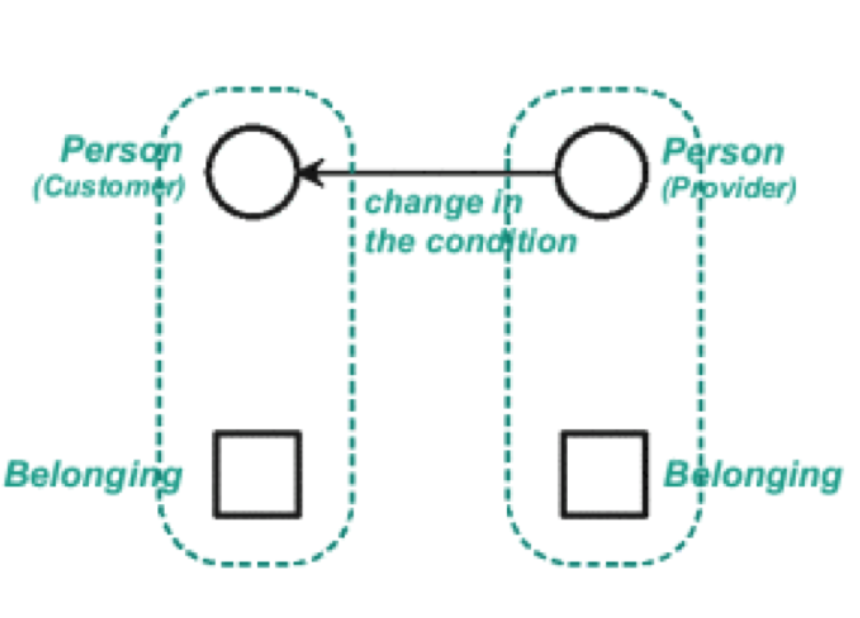
\includegraphics[width=150pt]{images/person-person}\hspace*{\fill}
  \label{fig:person-person}
\end{figure}\\ \\
\myparagraph{Person with belonging on person}
A person delivers a service to another person (e.g., haircut, medical service, teaching). Providers belongings (tools needed to provide the service) are used to deliver the service.
\begin{figure}[h!]
 \hfill 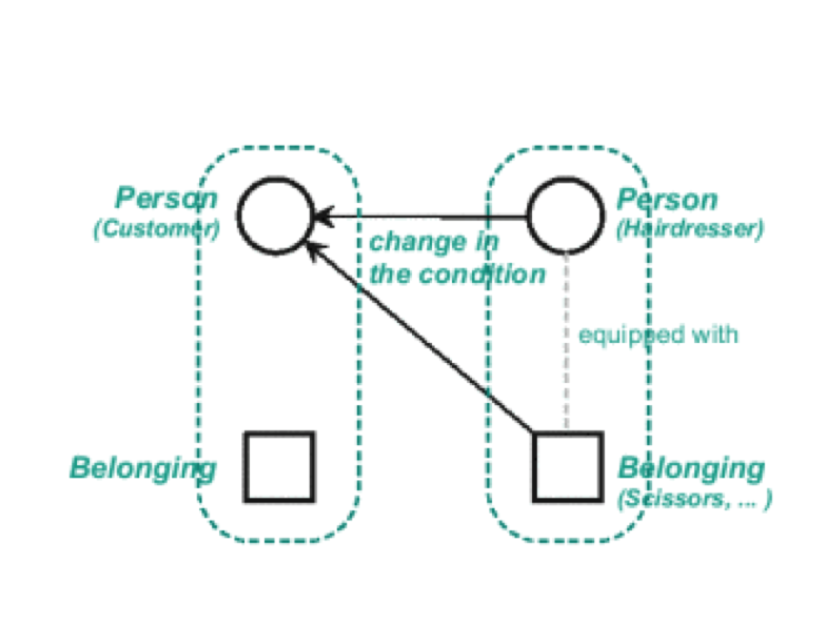
\includegraphics[width=150pt]{images/person-b-person}\hspace*{\fill}
  \label{fig:person-b-person}
\end{figure}
\myparagraph{Person with belonging acting on belonging}
A person delivers a service to another person changing the conditions of the customer belonging (e.g., car repair, transportation). Providers belongings (tools) are used to deliver the service. Customer belongings are managed by the provider.
\begin{figure}[h!]
 \hfill 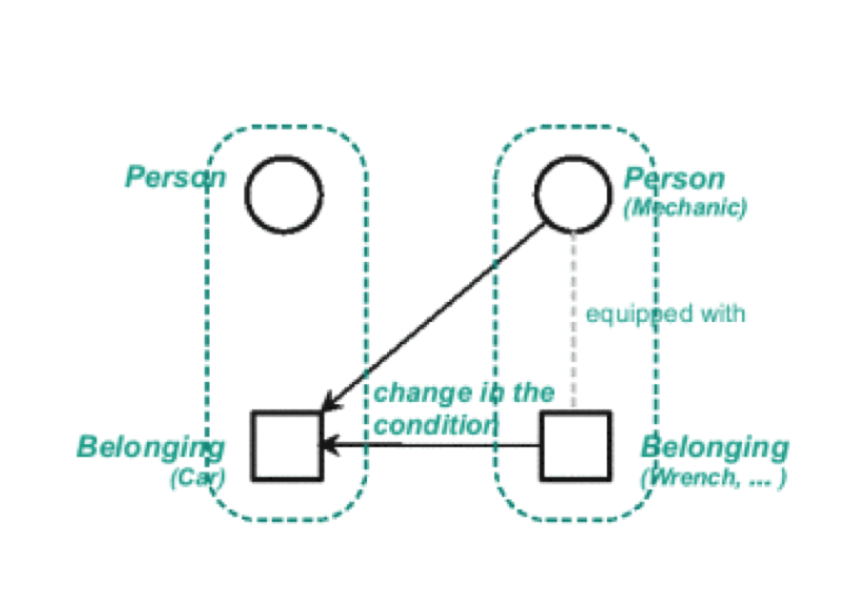
\includegraphics[width=150pt]{images/person-belonging}\hspace*{\fill}
  \label{fig:person-belonging}
\end{figure}
\myparagraph{Person acting on person}
Customer interacts with providers belonging to exploit a service (e.g., self-service). Providers belongings (tools) are used to deliver the service. Human intervention at provider side is limited. Customer needs to interact with machines (H2M). \\ 
Customer does not communicate with the service provider but he/she uses their belongings (e.g, Consumer uses the ATM without "seeing" the bank). 
\begin{figure}[h!]
 \hfill 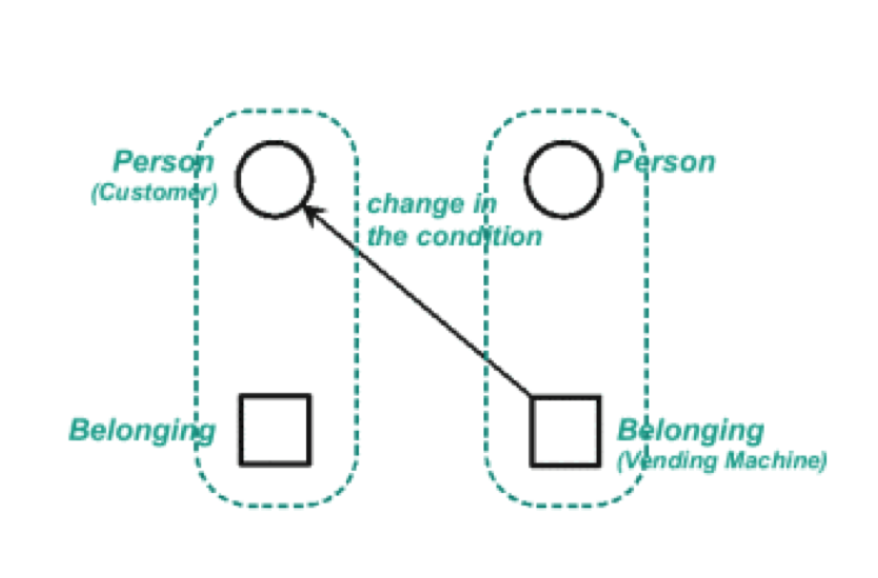
\includegraphics[width=150pt]{images/belonging-person}\hspace*{\fill}
  \label{fig:belonging-person}
\end{figure}
\myparagraph{Belonging acting on belonging}
Belongings are directly interacting (e.g., web services). Providers belongings (tools) are used to deliver the service. Human intervention at provider side is limited. Customer needs to be equipped with belonging able to communicate with the provider belonging (M2M). This is the case of a computer communicating with a web service.
\begin{figure}[h!]
 \hfill 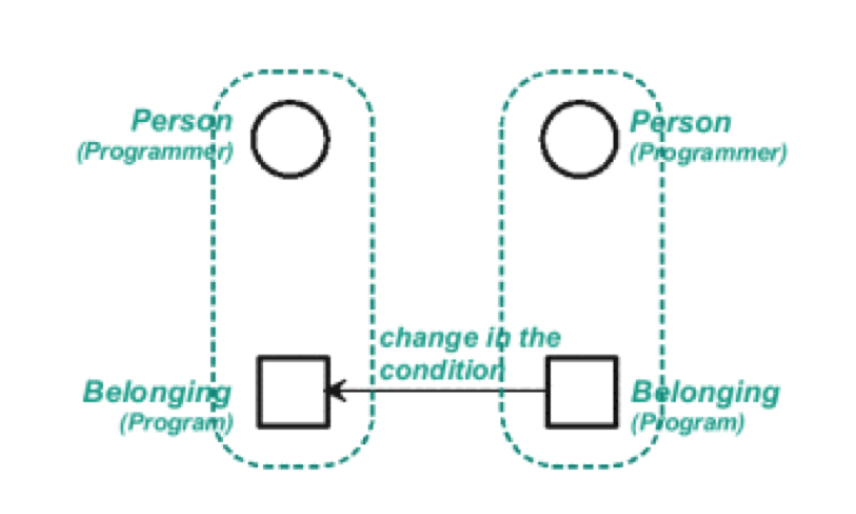
\includegraphics[width=150pt]{images/belonging-belonging}\hspace*{\fill}
  \label{fig:belonging-belonging}
\end{figure}
\subsubsection{Resource intensity of services}
Resource intensity is a measure of the resources required for the provision of a unit of a good or service.
\begin{itemize}
	\item \textbf{Labor- and capital-intensive services}: labor costs outweigh the costs for equipment and materials (e.g., hospital)
	\item \textbf{Knowledge-intensive services}: heavily rely on professional knowledge (e.g., medical doctors)
	\item \textbf{Information-intensive services}: activities are mainly focused on data management (e.g., data analytics)
	\item \textbf{Technology-intensive services}: labor costs becomes negligible (e.g., web service, cloud services)
\end{itemize}
\subsubsection{Technology in e-Services}
Technology can be used at (both) consumer and provider side in different ways and with different pervasiveness. Technology then, can assume different roles.
\begin{figure}[h!]
 \hfill 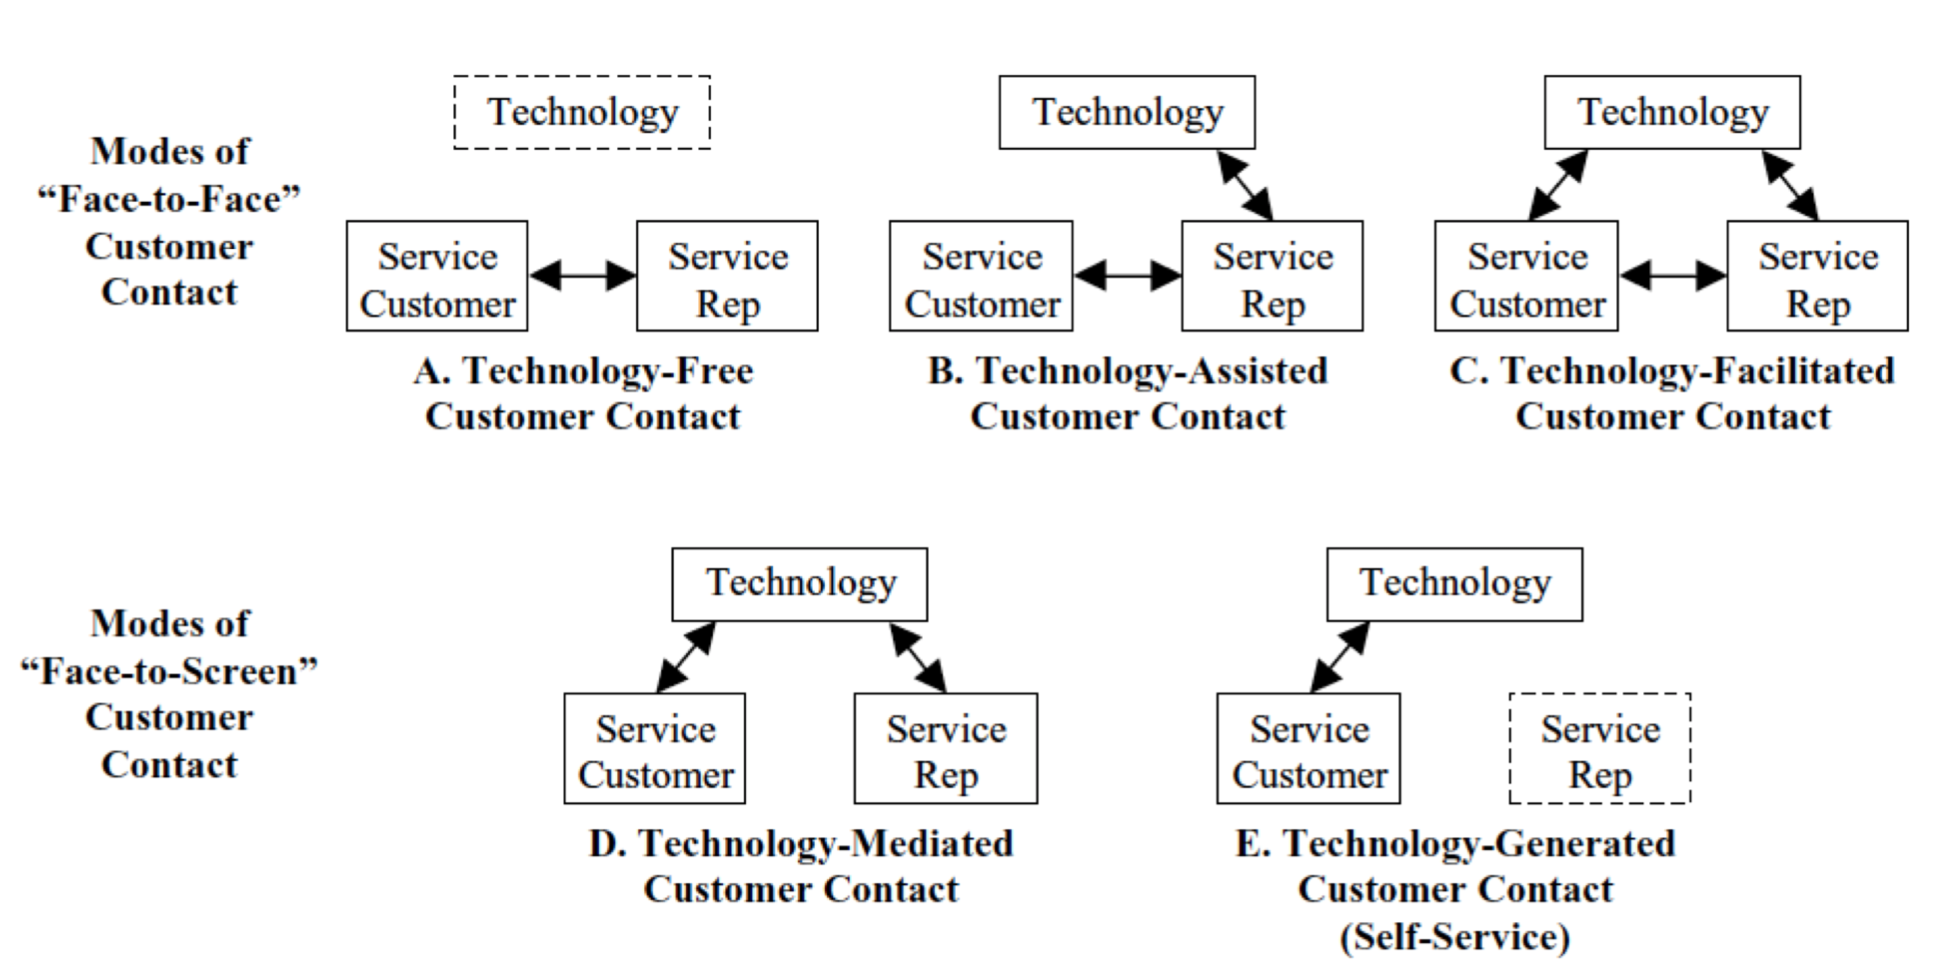
\includegraphics[width=200pt]{images/roles-tech}\hspace*{\fill}
 \caption{Possible roles of technology}
  \label{fig:roles-tech}
\end{figure}
\myparagraph{Face to face interaction}
Here services providers and service consumers are human beings. We distinguish:
\begin{itemize}
	\item \textbf{Technology-assisted services (e.g., bank teller)}:
	\begin{itemize}
		\item service consumer does not have access to the technology as the service provider acts as a mediator
		\item service provider uses technology to improve the interaction with the service consumer
	\end{itemize}
	\item \textbf{Technology-facilitated services (e.g., beamer)}:
		\begin{itemize}
		\item service provider uses technology to improve the interaction with the service consumer
		\item service consumer can have access to the technology together with the service provider
	\end{itemize}
\end{itemize}
\myparagraph{Face to screen interaction}
Here technology is in the middle between providers and consumers (e.g., telephone,web). These below by definitions are e-Services.
\begin{itemize}
	\item \textbf{Technology-mediate services}:
	\begin{itemize}
		\item service providers and consumers are human beings
		\item e.g., call center, Amazon Mechanical Turk
	\end{itemize}
	\item \textbf{Technology-generated services}:
		\begin{itemize}
		\item service providers are replaced by technology
		\item e.g., ATM, home banking
	\end{itemize}
\end{itemize}
\subsubsection{e-Services}
\textit{"An electronic service, a.k.a. e-Service, is a service system (with elements, a structure, a behavior, and a purpose) for which the implementation of many of this elements and behavior is done using automation and programming techniques."} \\(J. Cardoso, Fundamentals of Service Systems)
\myparagraph{The value of e-Services}
\begin{itemize}
	\item \textbf{Accessibility}: services can be accessed almost everywhere. Now the communication infrastructure is now available everywhere since the adoption of smartphone is covering the majority of population.
	\item \textbf{Delivery}: delivery is almost instantaneous, but it depends on the nature of the service (ATM vs. booking)
	\item \textbf{Human touch}: customer experience is one of the main drawbacks of e-Services adoption, that's why technology is trying to reduce this gap through UX studies
	\item \textbf{Personalization}: one-to-one relationship is fundamental, private data need to be share
\end{itemize}
The e-Service provisioning is usually driven by a business process. The customer of the service is one of the parties involved in the business process. The business process, to be enacted, could be based on other services: some of them human-based; some of them automatic (more interesting for us).
\begin{figure}[ht!]
 \hfill 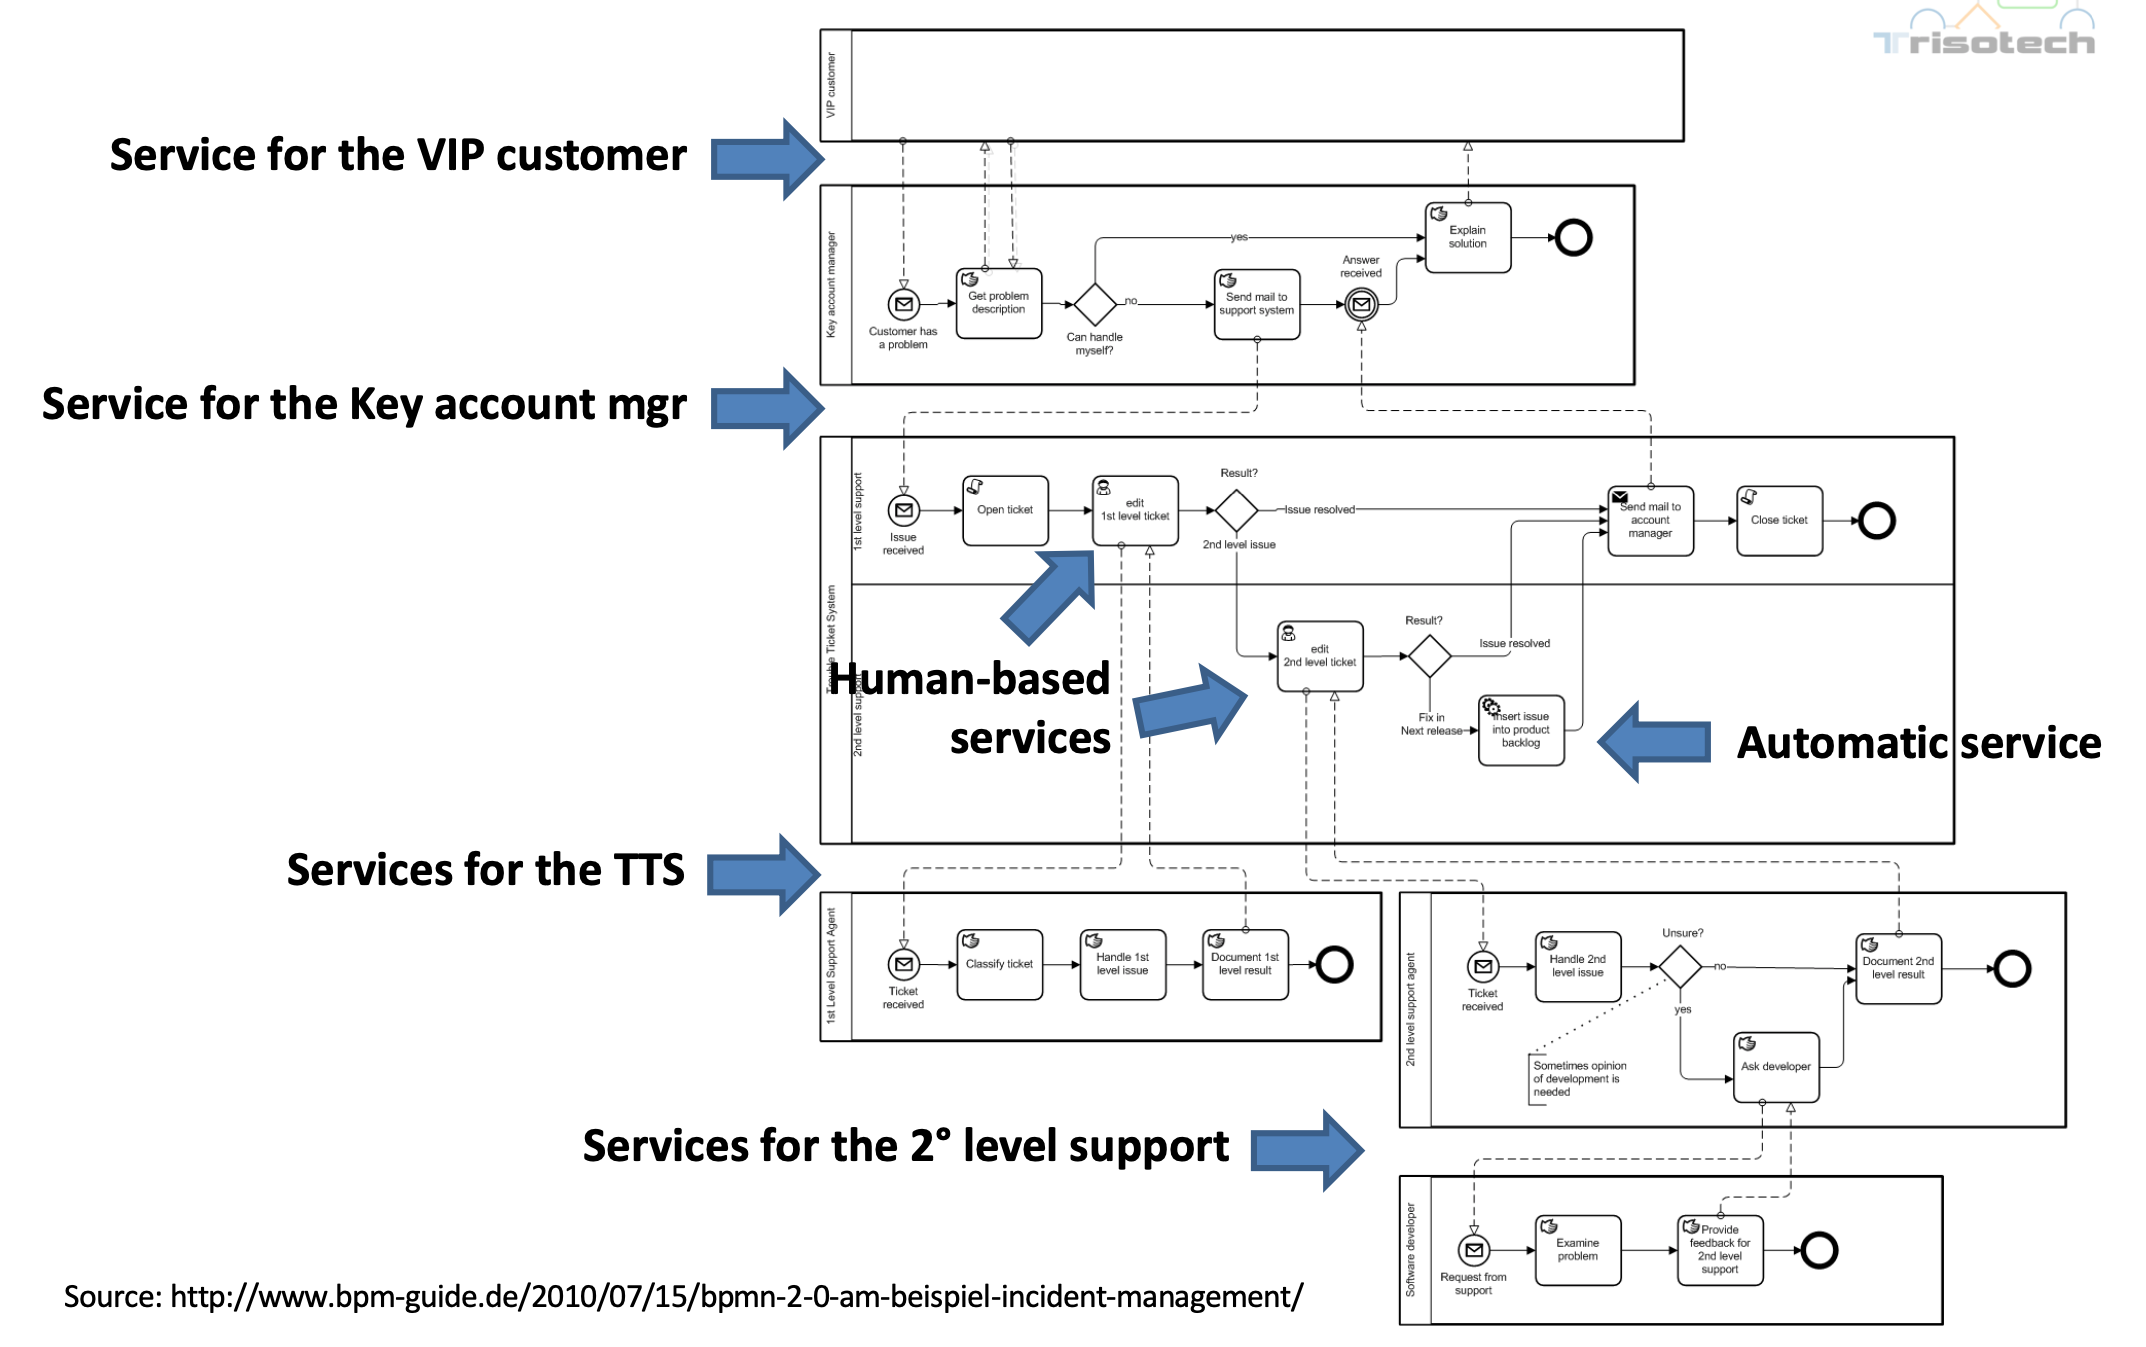
\includegraphics[width=\linewidth]{images/business-process}\hspace*{\fill}
 \caption{BPM Collaboration diagram}
  \label{fig:business-process}
\end{figure} \\
Figure 12 shows an example of BPM collaboration diagram in which different services and processes collaborate at different levels in order to provide a complex service. 
\pagebreak
\section{|LARGE Service Blueprint}
\subsection{Service design}
Service design is design for experiences that reach people through many different touch points, and that happen over time. It is composed by a set of methods and principles coming from different disciplines which are systematically applied to the creation of new services (Interaction designers, Information science, Management science, ...)
\subsubsection{Service design principles}
\begin{itemize}
	\item \textbf{Human-centered}: everything starts from a deep understanding of the needs of the users. \textcolor{MidnightBlue}{Designing our services based upon how they are experienced from the ‘customer’s perspective.’} Placing the user or consumer in the centre of the service allows us to discover how the patient experiences the service. We do this by implementing a range of techniques including interviews, observations and field research to gather insights into the consumer’s needs, experiences and behaviours.
	\item \textbf{Co-designed}: service innovation is not possible without the acceptance of all stakeholders. \textcolor{MidnightBlue}{All stakeholder groups should be involved in the service design process.} Co-creation is the process of involving users not only in the design of the solution but also the production and development of it. Multidisciplinary teams from all levels within our organisation will allow for a range of expertise, knowledge and skills and will generate great ideas. Work out who is within the service ‘ecosystem’ and make sure every party is represented.
	\item \textbf{Sequenced}: services must be designed as dynamic processes that take place over time. 
	\item \textbf{Holistic}: all the aspects of the service, both digital and physical should be considered. \textcolor{MidnightBlue}{The entire environment in which the service exists and is delivered should be considered.} Holistic services look at the whole user journey and consider each touch point of that service. Touchpoints refer to any interactions that occur between users and a service. A holistic approach can be achieved by using service blue prints, personas or fictional characters to highlight different user experiences and user journeys. A well-rounded and complete service also involves the functionality, safety and reliability of the service.
	\item \textbf{Evidenced}: visualize and prototype our service concept early and often. \textcolor{MidnightBlue}{In a collaborative team environment, it is more expressive to use visual aids than to rely purely on words. }Get the team to use sketches, pictures, graphs, maps and prototypes where applicable. Be creative with coloured pens and glue. Visual tools can be less complicated to digest and more tangible. They make things easier to remember and can help to properly explain what we’re trying to achieve.
	\item \textbf{Agile}: Our process is incremental and iterative: start small, test early and learn quickly from failure and success. \textcolor{MidnightBlue}{One of the main features of services design is not avoiding making mistakes but learning from them.} This is achieved by prototyping and testing. You can save a large amount of time and money if we test the experience before spending lengthy periods of time developing it. It’s imperative to prototype solutions before we launch them but it is also a good idea to release and test our iterations many times through the process. Don’t just wait until the end of the project to do so.
\end{itemize}
\pagebreak
\begin{figure}[ht!]
 \hfill 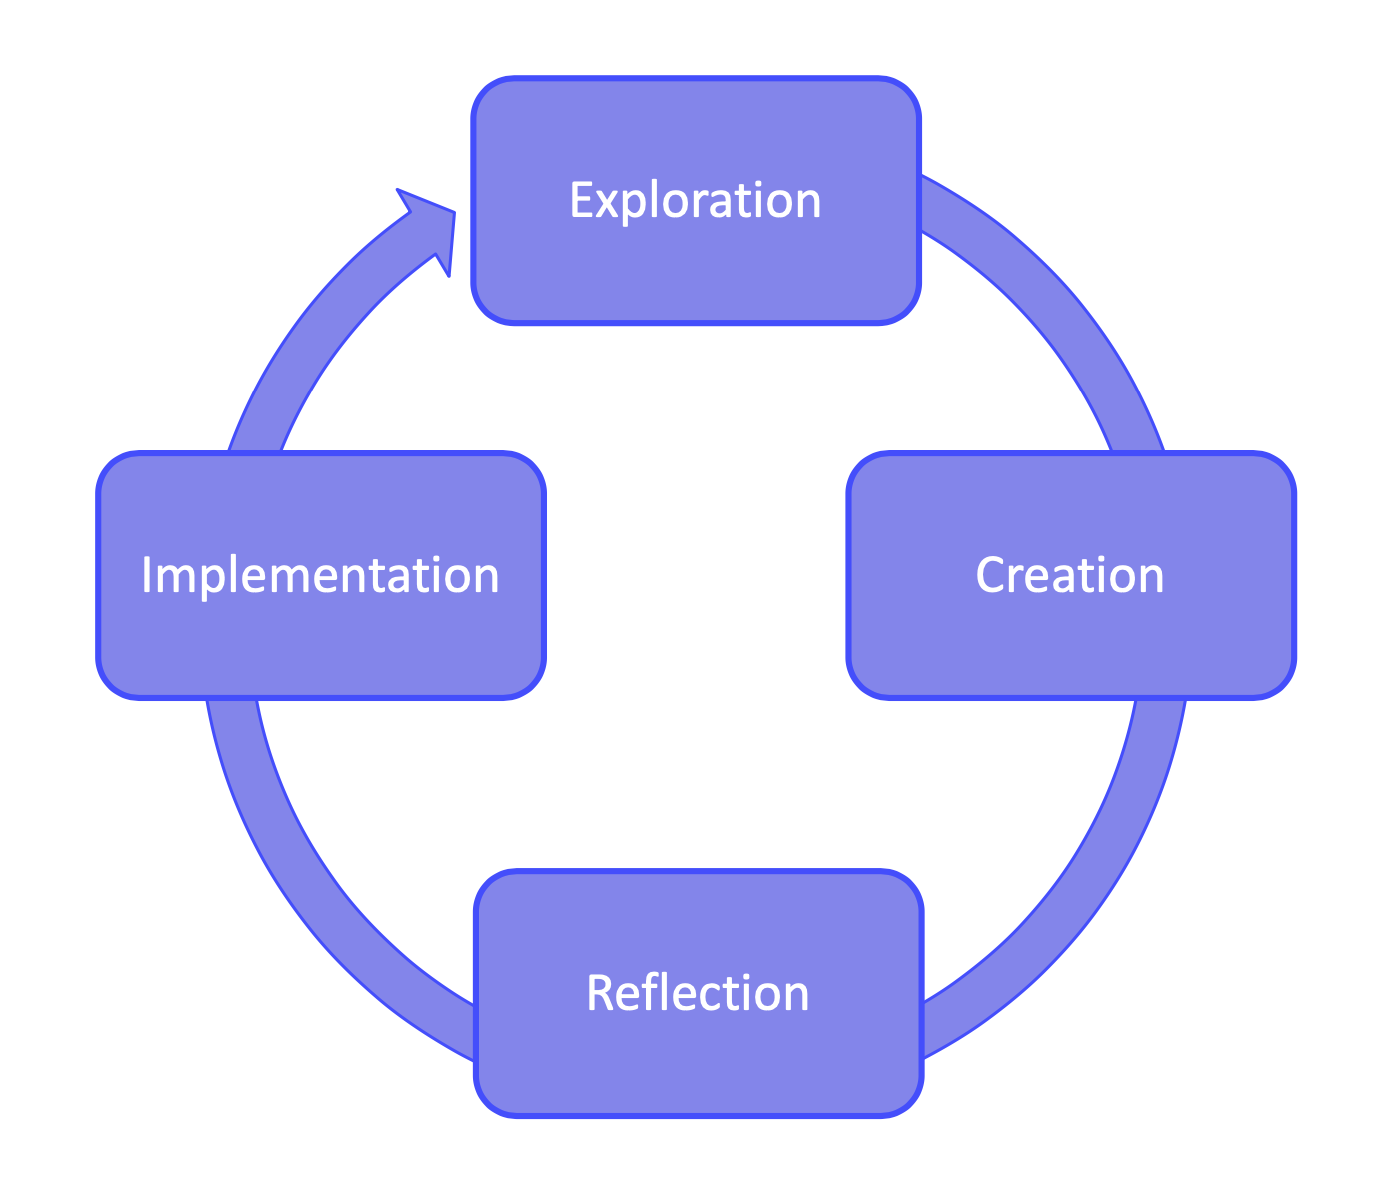
\includegraphics[width=200pt]{images/service-design-process}\hspace*{\fill}
 \caption{Service design process}
  \label{fig:service-design-process}
\end{figure}
Each of the phases in Figure 13 consists in different activities.
\begin{figure}[ht!]
 \hfill 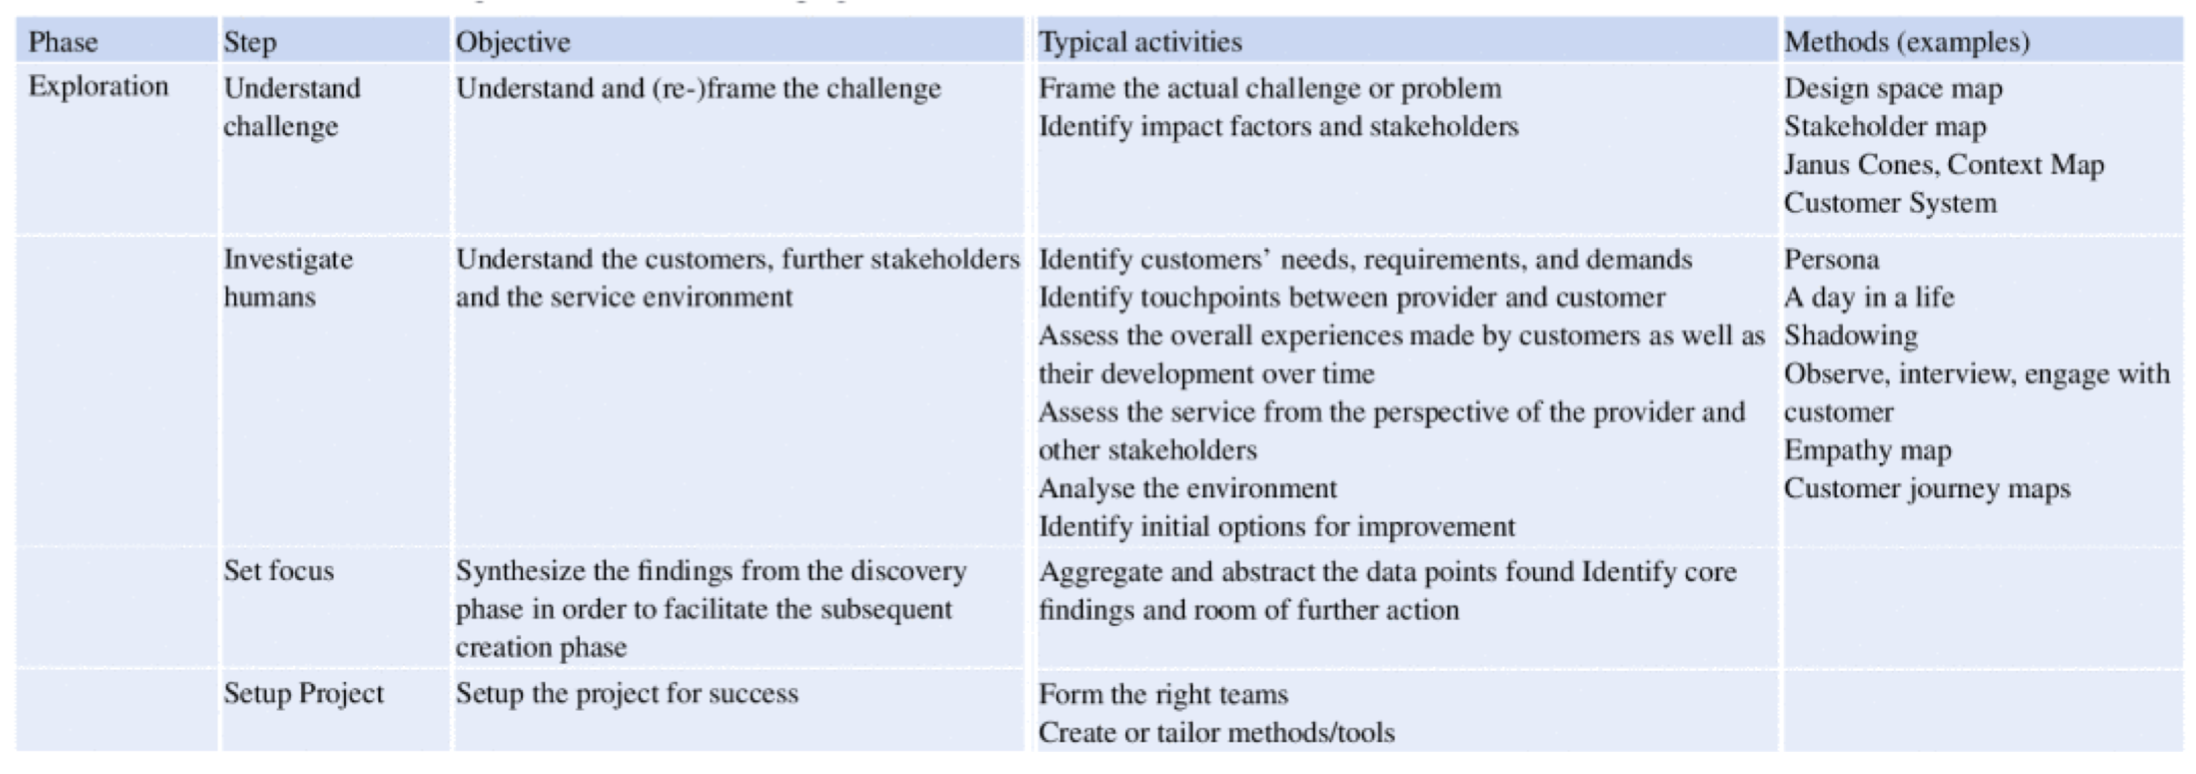
\includegraphics[width=410pt]{images/exploration}\hspace*{\fill}
 \caption{Exploration phase}
  \label{fig:exploration}
\end{figure}
\begin{figure}[ht!]
 \hfill 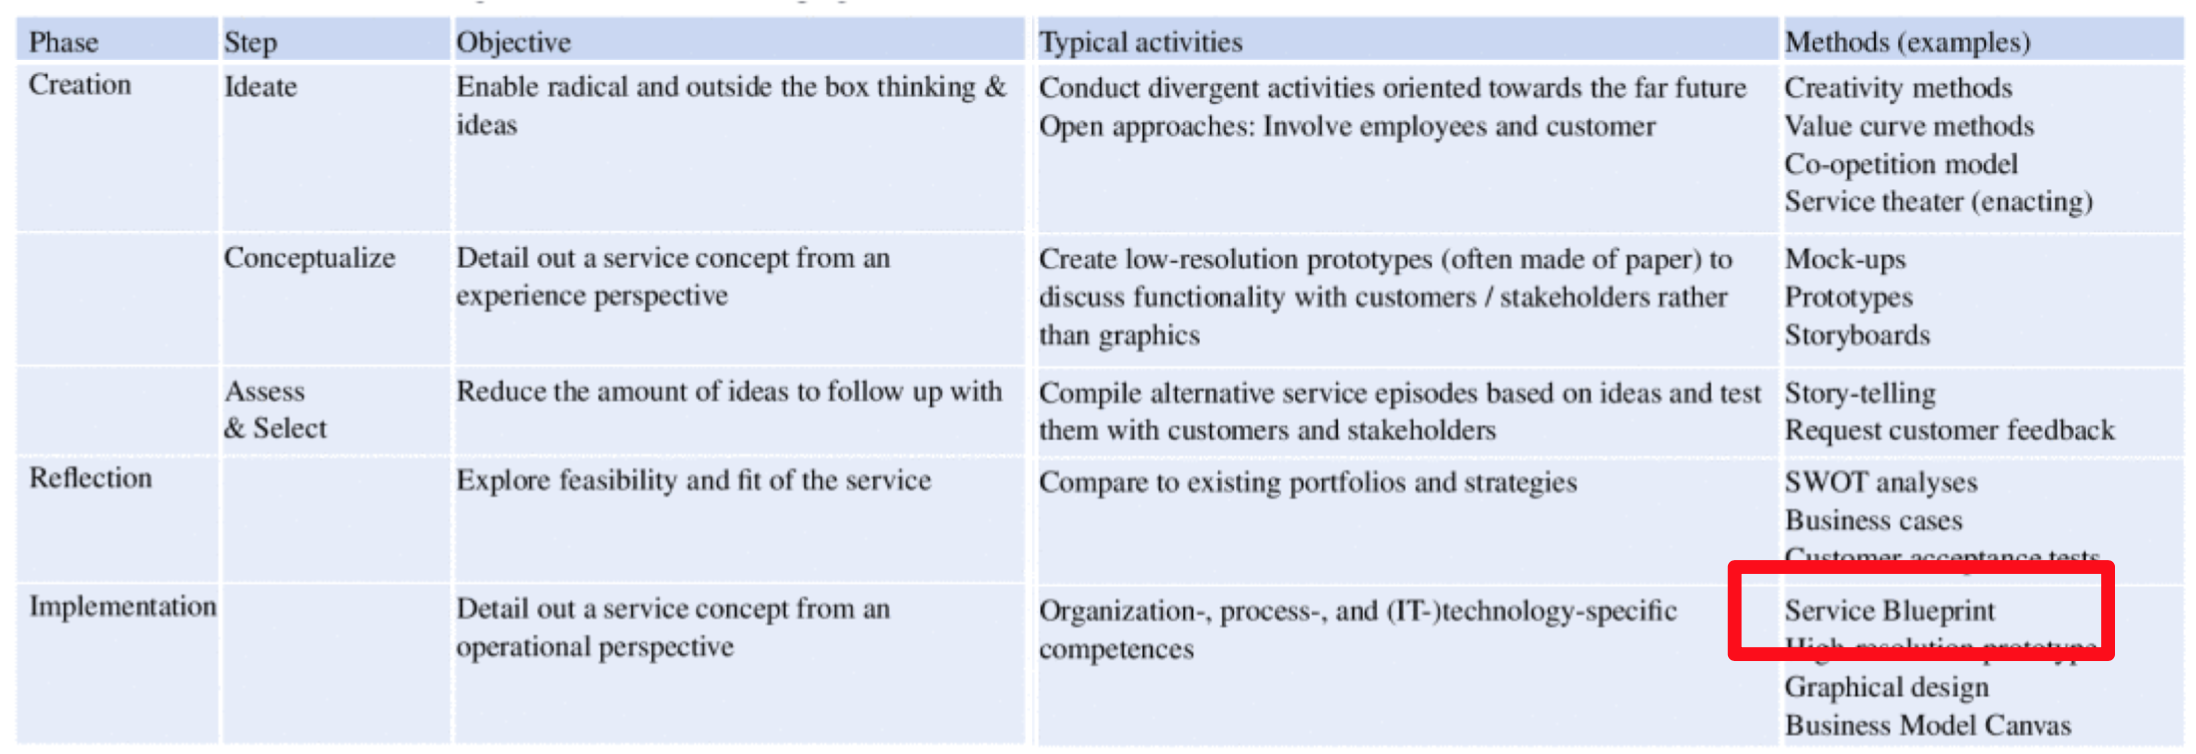
\includegraphics[width=410pt]{images/other-phases}\hspace*{\fill}
 \caption{Creation, Reflection and Implementation}
  \label{fig:other-phases}
\end{figure}
\subsection{Service blueprinting}
A \textbf{service blueprint} describes how a company delivers service to customers in order to improve customers' and employees’ experience. It is also used to plan and organize resources: people, tools and processes. \\ \\
\textbf{Service blueprinting} is Technique to help organizations understanding their service offering (or designing new services) and delivery processes by enabling to examine service processes from a customers point of view. The result is a graphical representation, i.e., map, of:
\begin{itemize}
	\item The user journey (phase by phase, step by step)
	\item The touchpoints (channel by channel, touchpoint by touchpoint)
	\item The backstage processes (stakeholder by stakeholder, action by action)
\end{itemize}
\uline{The definition of a blueprint usually requires a team work.} \\ \\
Why do we need a service blueprint?  \\
It helps changing perspective. The main question is not how a service is delivered (still relevant). \textbf{The main questions are what is delivered}. It is about framing problem before solving it. 
\\ 
For example, Mc Donald, is an highly designed service:
\begin{itemize}
	\item What you obtain
	\item The time in which you obtain goods
	\item The experience (what the employees say)
\end{itemize}
\pagebreak
\begin{figure}[ht!]
 \hfill 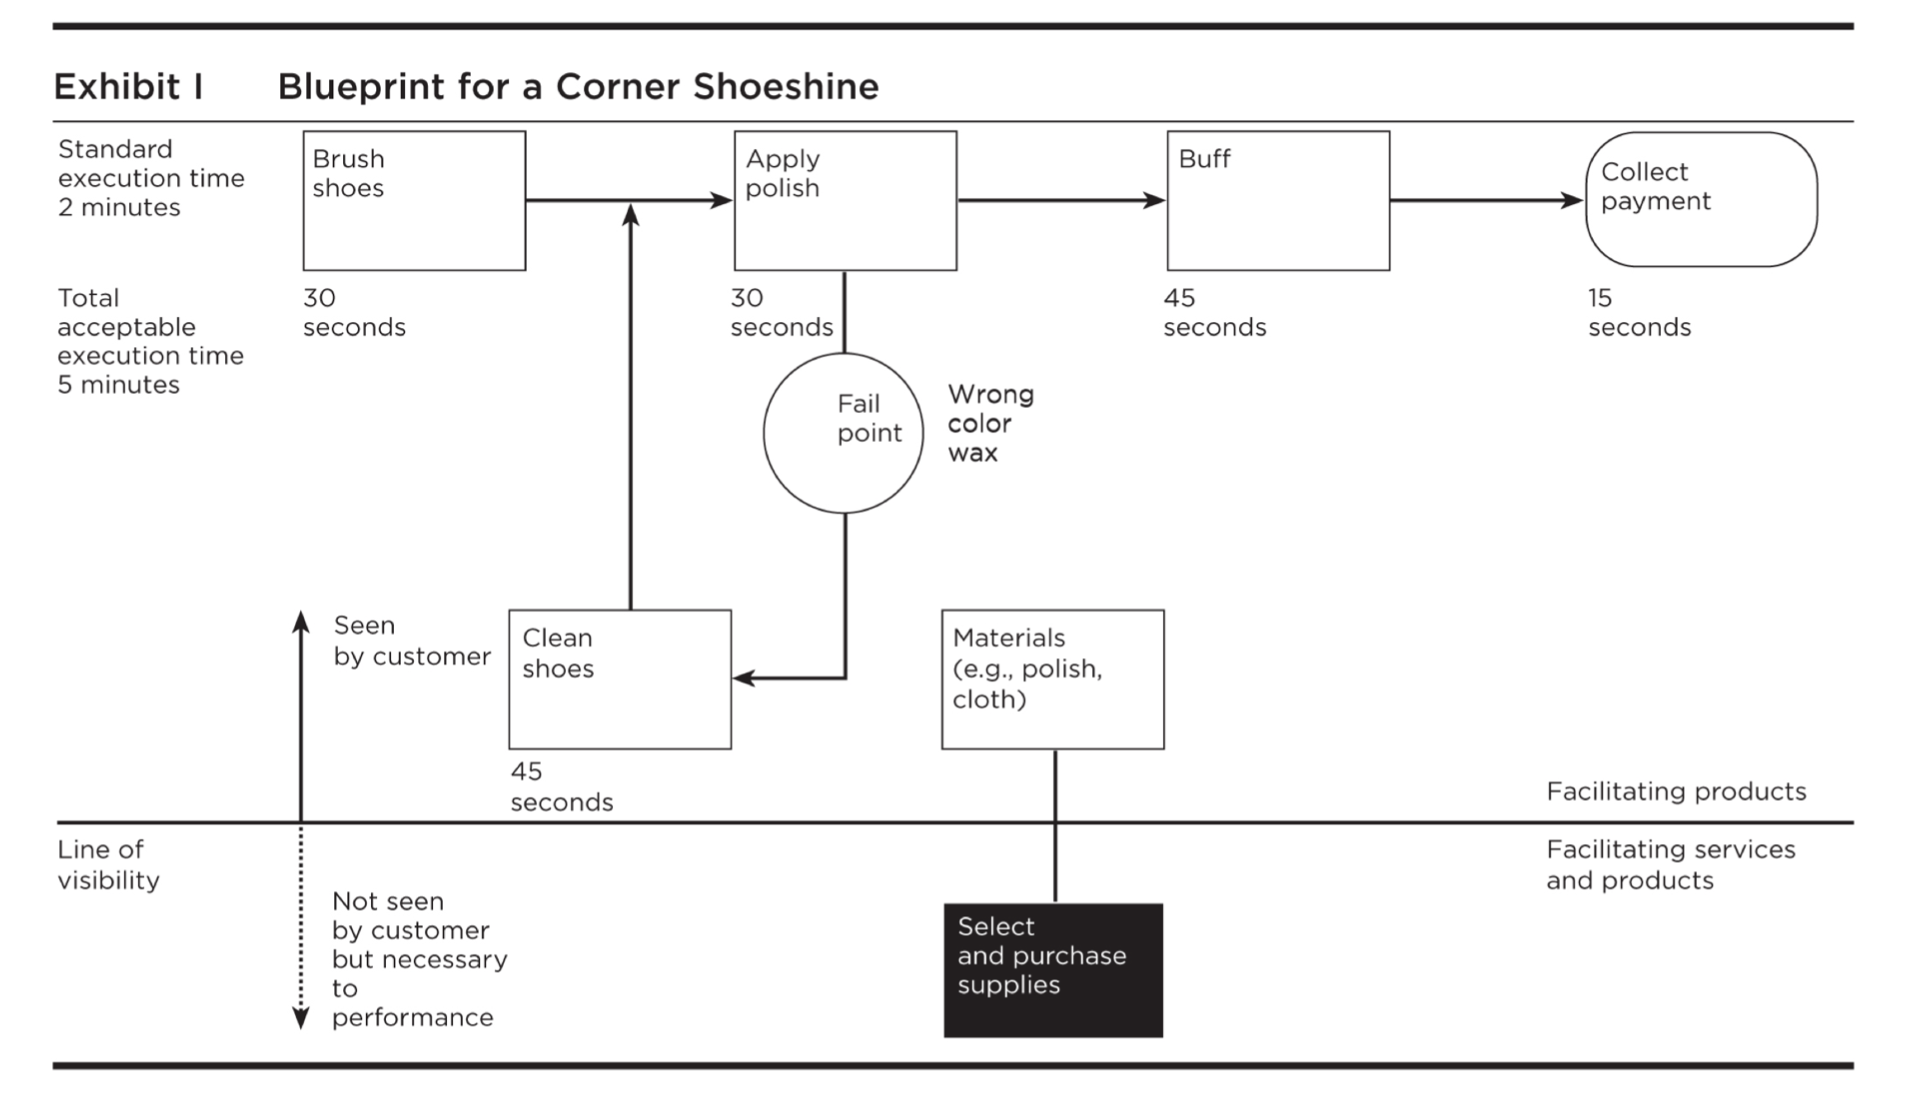
\includegraphics[width=350pt]{images/first-blueprint}\hspace*{\fill}
 \caption{First blueprint example}
  \label{fig:first-blueprint}
\end{figure}
\textit{!Note that there exists no standard blueprint, every domain has its own.} 
\\ \\
Figure 17 shows an example blueprint for a Corner Shoeshine. The line of visibility separates what is visible to the consumer (upper part) from what is visible only to the service provider.
\begin{figure}[ht!]
 \hfill 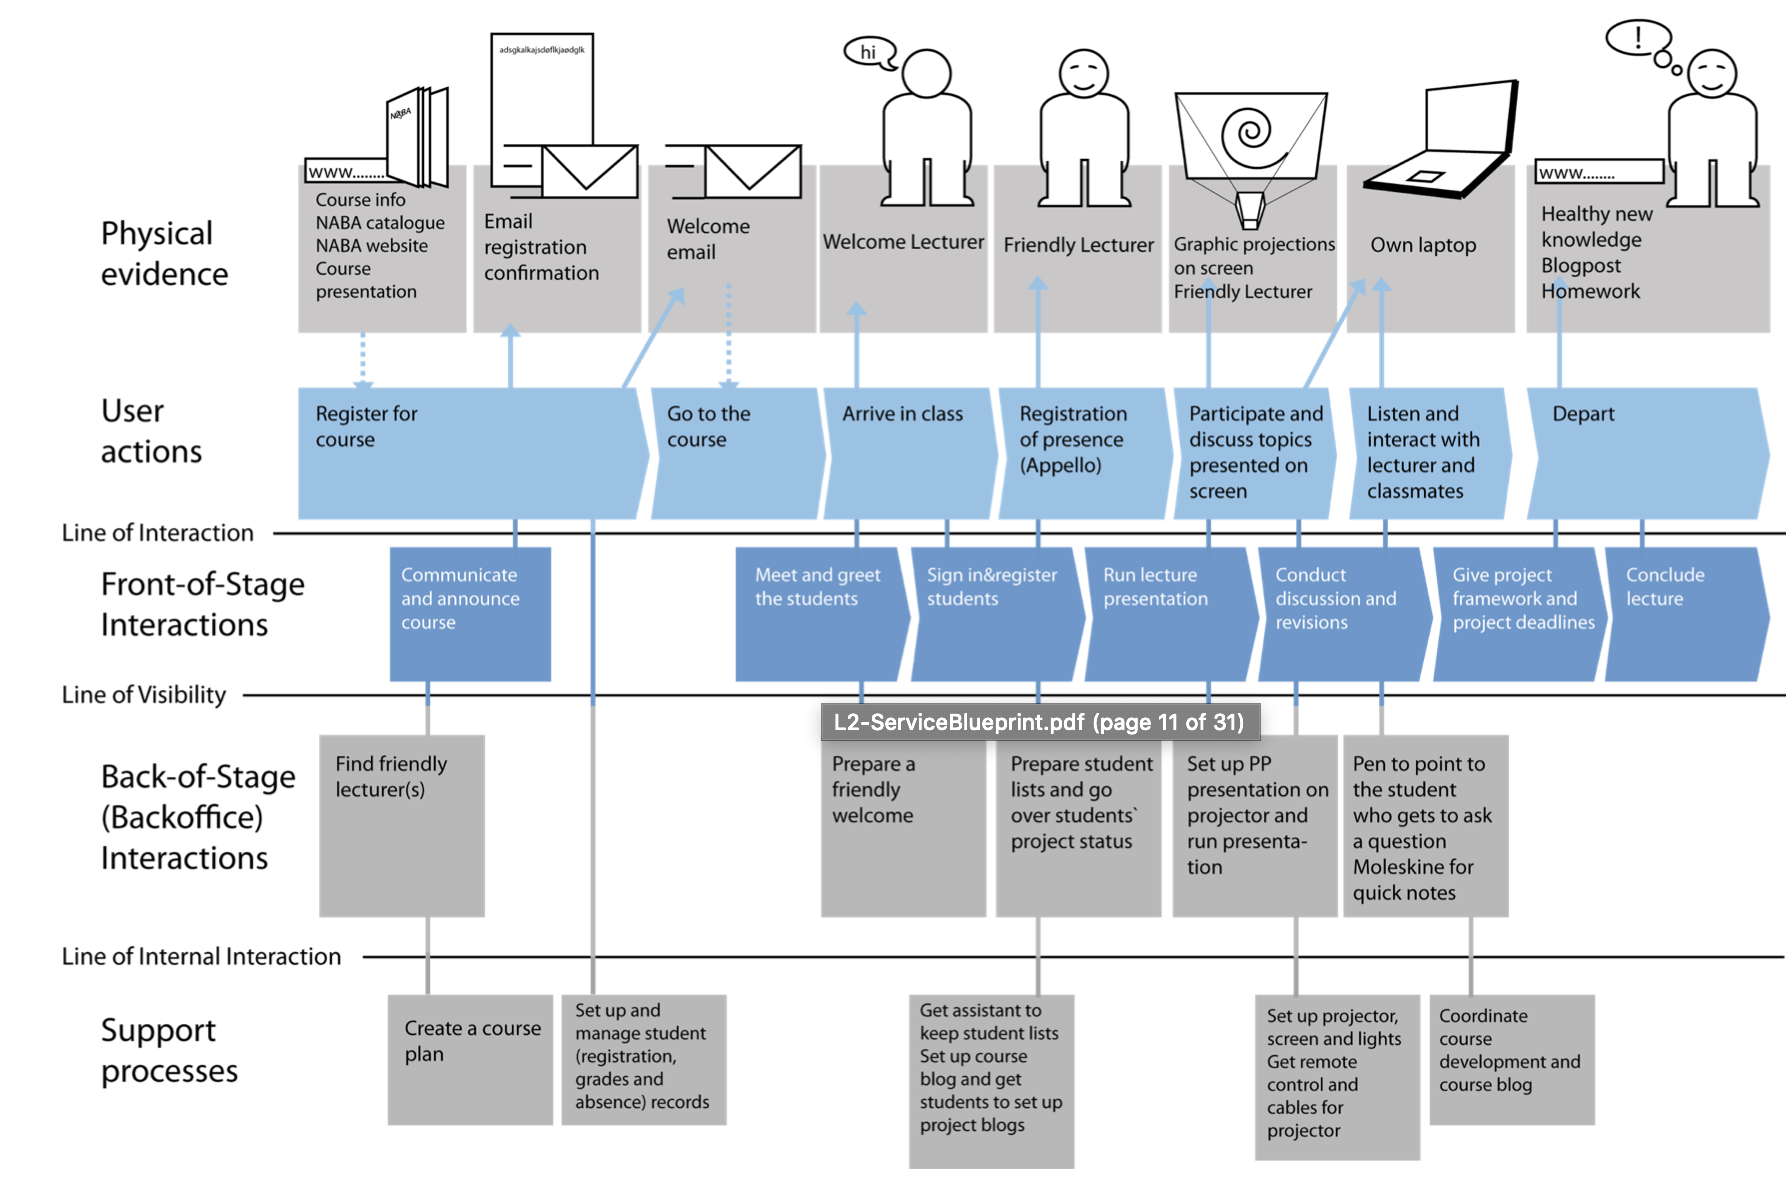
\includegraphics[width=400pt]{images/second-service-blueprint}\hspace*{\fill}
 \caption{Second blueprint example}
  \label{fig:second-blueprint}
\end{figure}
\clearpage
\section{\LARGE References}
\begin{enumerate}[label={[\arabic*]}]
  \item C. M. MacKenzie et al.,Reference Model for Service Oriented
Architecture 1.0., OASIS Open, 2006
\end{enumerate}
\end{document}